%%%%%%%%%%%%%%%%%%%%%%%%%%%%%%%%%%%%%%%%%%%%%%%%%%%%%%%%%%%%%%%%%%%%%%%%%%%%
% AGUJournalTemplate.tex: this template file is for articles formatted with LaTeX
%
% This file includes commands and instructions
% given in the order necessary to produce a final output that will
% satisfy AGU requirements, including customized APA reference formatting.
%
% You may copy this file and give it your
% article name, and enter your text.
%
% guidelines and troubleshooting are here: 

%% To submit your paper:
\documentclass[draft]{agujournal2019}
\usepackage{url} %this package should fix any errors with URLs in refs.
\usepackage{lineno}
\usepackage[inline]{trackchanges} %for better track changes. finalnew option will compile document with changes incorporated.
\usepackage{soul}
\linenumbers
%%%%%%%
% As of 2018 we recommend use of the TrackChanges package to mark revisions.
% The trackchanges package adds five new LaTeX commands:
%
%  \note[editor]{The note}
%  \annote[editor]{Text to annotate}{The note}
%  \add[editor]{Text to add}
%  \remove[editor]{Text to remove}
%  \change[editor]{Text to remove}{Text to add}
%
% complete documentation is here: http://trackchanges.sourceforge.net/
%%%%%%%

% \draftfalse

%% Enter journal name below.
%% Choose from this list of Journals:
%
% JGR: Atmospheres
% JGR: Biogeosciences
% JGR: Earth Surface
% JGR: Oceans
% JGR: Planets
% JGR: Solid Earth
% JGR: Space Physics
% Global Biogeochemical Cycles
% Geophysical Research Letters
% Paleoceanography and Paleoclimatology
% Radio Science
% Reviews of Geophysics
% Tectonics
% Space Weather
% Water Resources Research
% Geochemistry, Geophysics, Geosystems
% Journal of Advances in Modeling Earth Systems (JAMES)
% Earth's Future
% Earth and Space Science
% Geohealth
%
% ie, \journalname{Water Resources Research}

\journalname{JGR: Oceans}


\begin{document}

%%%%%%%%%%%%%%%%%%%%%%%%%%%%%%%%%%%%%%%%%%%%%%%
%  TITLE
%
% (A title should be specific, informative, and brief. Use
% abbreviations only if they are defined in the abstract. Titles that
% start with general keywords then specific terms are optimized in
% searches)
%
%%%%%%%%%%%%%%%%%%%%%%%%%%%%%%%%%%%%%%%%%%%%%%%

% Example: \title{This is a test title}

\title{Evidence of Synoptic Cross-shelf Pathways of Mid-depth Salinity Maximum Intrusions in the South Brazil Bight}

%%%%%%%%%%%%%%%%%%%%%%%%%%%%%%%%%%%%%%%%%%%%%%%
%
%  AUTHORS AND AFFILIATIONS
%
%%%%%%%%%%%%%%%%%%%%%%%%%%%%%%%%%%%%%%%%%%%%%%%

% Authors are individuals who have significantly contributed to the
% research and preparation of the article. Group authors are allowed, if
% each author in the group is separately identified in an appendix.)

% List authors by first name or initial followed by last name and
% separated by commas. Use \affil{} to number affiliations, and
% \thanks{} for author notes.
% Additional author notes should be indicated with \thanks{} (for
% example, for current addresses).

% Example: \authors{A. B. Author\affil{1}\thanks{Current address, Antartica}, B. C. Author\affil{2,3}, and D. E.
% Author\affil{3,4}\thanks{Also funded by Monsanto.}}

\authors{D. A. Silva\affil{1}, A. Gangopadhyay\affil{2}, D. K. Sasaki\affil{3}, M. Dottori\affil{1}, I. C. A. Silveira\affil{1}, W. C. Belo\affil{4}, R. P. Martins\affil{4}}

\affiliation{1}{Instituto Oceanogr\'{a}fico, Universidade de Sao Paulo, Praca do Oceanogr\'{a}fico, 191 - SP 05508-120, S\~{a}o Paulo, Brasil}
\affiliation{2}{School for Marine Sciences and Technology, University of Massachusetts, 836 South Rodney French Blvd, New Bedford, MA 02744-1221}
\affiliation{4}{Department of Marine and Environmental Sciences, Northeatern University, 430 Nahant Rd, Nahant, MA 01908}
\affiliation{3}{Centro de Pesquisas, Desenvolvimento e Inova\c{c}\~{a}o Leopoldo Am\'{e}rico Miguez de Mello - CENPES/PETROBRAS, Av. Hor\'{a}cio Macedo, 950 - Cidade Universit\'{a}ria da Universidade Federal do Rio de Janeiro, Rio de Janeiro - RJ, 21941-915}

%(repeat as many times as is necessary)


% Corresponding author mailing address and e-mail address:

% (include name and email addresses of the corresponding author.  More
% than one corresponding author is allowed in this LaTeX file and for
% publication; but only one corresponding author is allowed in our
% editorial system.)

% Example: \correspondingauthor{First and Last Name}{email@address.edu}

\correspondingauthor{Danilo Silva}{danilo2.silva@usp.br}



%%%%%%%%%%%%%%%%%%%%%%%%%%%%%%%%%%%%%%%%%%%%%%%
% KEY POINTS
%%%%%%%%%%%%%%%%%%%%%%%%%%%%%%%%%%%%%%%%%%%%%%%
%  List up to three key points (at least one is required)
%  Key Points summarize the main points and conclusions of the article
%  Each must be 140 characters or fewer with no special characters or punctuation and must be complete sentences

% Example:
% \begin{keypoints}
% \item	List up to three key points (at least one is required)
% \item	Key Points summarize the main points and conclusions of the article
% \item	Each must be 140 characters or fewer with no special characters or punctuation and must be complete sentences
% \end{keypoints}

\begin{keypoints}
\item Observational evidence of remotely advected Salinity Maximum intrusions (\textit{$S_{max}$}) in the Northeastern South Brazil Bight (NE-SBB) from a multi-platform observational dataset
\item Pathways from the dataset indicate remotely advected intrusions from the east and north of NE-SBB.
\item Wind and eddy-driven circulation are linked to the identified pathways.
\end{keypoints}

%%%%%%%%%%%%%%%%%%%%%%%%%%%%%%%%%%%%%%%%%%%%%%%
%
%  ABSTRACT and PLAIN LANGUAGE SUMMARY
%
% A good Abstract will begin with a short description of the problem
% being addressed, briefly describe the new data or analyses, then
% briefly states the main conclusion(s) and how they are supported and
% uncertainties.

% The Plain Language Summary should be written for a broad audience,
% including journalists and the science-interested public, that will not have 
% a background in your field.
%
% A Plain Language Summary is required in GRL, JGR: Planets, JGR: Biogeosciences,
% JGR: Oceans, G-Cubed, Reviews of Geophysics, and JAMES.
% see http://sharingscience.agu.org/creating-plain-language-summary/)
%
%%%%%%%%%%%%%%%%%%%%%%%%%%%%%%%%%%%%%%%%%%%%%%%

%% \begin{abstract} starts the second page

\begin{abstract}
Cross-shelf exchanges play a crucial role in the distribution of heat, salt, pollutants, and biogeochemical properties between the continental shelf and the open ocean. Among the various processes that shape these exchanges, the intrusion of salty and warm waters (known as salinity maximum intrusions, \textit{$S_{max}$}) remains poorly understood in the South Brazil Bight (SBB). This study provides evidence of Smax intrusions from independent observations made between February and March 2022 in the Northeast SBB (NE-SBB). These intrusions resembled structures previously observed in several hydrographic campaigns. The dataset indicated an advective cross-shelf pathway as the primary route for these intrusions, originating from southeastern locations under geostrophic influence, captured by a Brazil Current meander, and further advected toward the shelf edge. Lagrangian analysis confirmed this pathway and suggested an additional along-shelf pathway, resembling the non-meandering state of the Brazil Current. Burger number (Bu) analysis revealed that wind-driven cross-shelf circulation over the shelf resulted in an onshore counterflow at mid-depths (Bu $>$ 1), which was enhanced by mesoscale dynamics associated with the Brazil Current system. Further research is needed to explore the interplay of processes driving \textit{$S_{max}$} onto the shelf. Nonetheless, these findings shed light on these structures and underscore the importance of considering remote influences on the biogeochemical processes of the SBB.
\end{abstract}

\section*{Plain Language Summary}
This study examines the movement of warm, salty water (Salinity Maximum intrusions, \textit{$S_{max}$}) between the continental shelf and the open ocean in the South Brazil Bight (SBB). In early 2022, researchers observed these water intrusions in the northeastern SBB, noting that they primarily travel across the shelf from the southeast, influenced by the Brazil Current. Additionally, some of this water also moves along the shelf. Wind-driven currents create an onshore flow at subsurface levels, which is strengthened by the Brazil Current's dynamics. These findings provide new insights into water movement in the SBB and its impact on marine processes, highlighting the need for further research to better understand these mechanisms.

%%%%%%%%%%%%%%%%%%%%%%%%%%%%%%%%%%%%%%%%%%%%%%%
%
%  BODY TEXT
%
%%%%%%%%%%%%%%%%%%%%%%%%%%%%%%%%%%%%%%%%%%%%%%%

\section{Introduction}
\label{sec:introduction}

Cross-shelf exchanges are critical processes that influence the distribution of heat, salt, pollutants \cite{brink2016} and biogeochemical properties \cite{liu2010carbon,cossarini2015continental} between the continental shelf and the open ocean. Western boundary currents (WBCs), such as the Brazil Current (BC), play an important role in these exchanges due to their dynamic nature and the transport of warm, saline waters poleward along the western margins of ocean basins. 

The Northeastern South Brazil Bight (NE-SBB, Figure~\ref{fig:study_area}) exhibits a secondary maximum of eddy kinetic energy (eKE) in the South Atlantic Basin \cite<refer to Figure 1 from >{rocha2022}. This elevated eKE is linked to the quasi-permanent presence of cyclonic eddies generated off Cabo Frio (Cabo Frio Eddy, CFE) and Cabo de São Tomé (Cabo de São Tomé Eddy, CTE) \cite{uchoa2023,silveira2023}. The generation of these eddies results from the topographic interactions of the poleward BC and the equatorward Intermediate Western Boundary Current \cite{luko2022}. The development of meanders and cyclonic eddies influences cross-shelf exchanges \cite{calil2021,combes2023circulation}, in addition to wind-driven cross-shelf circulation \cite{castro2014summer,brink2016}. The on-shelf outcome of these processes over the shelf edge leads to the development of thermohaline intrusions, i.e., temperature and salinity inversions \cite{ruddick-kerr2003}.

\begin{figure}[ht!]
    \centering
    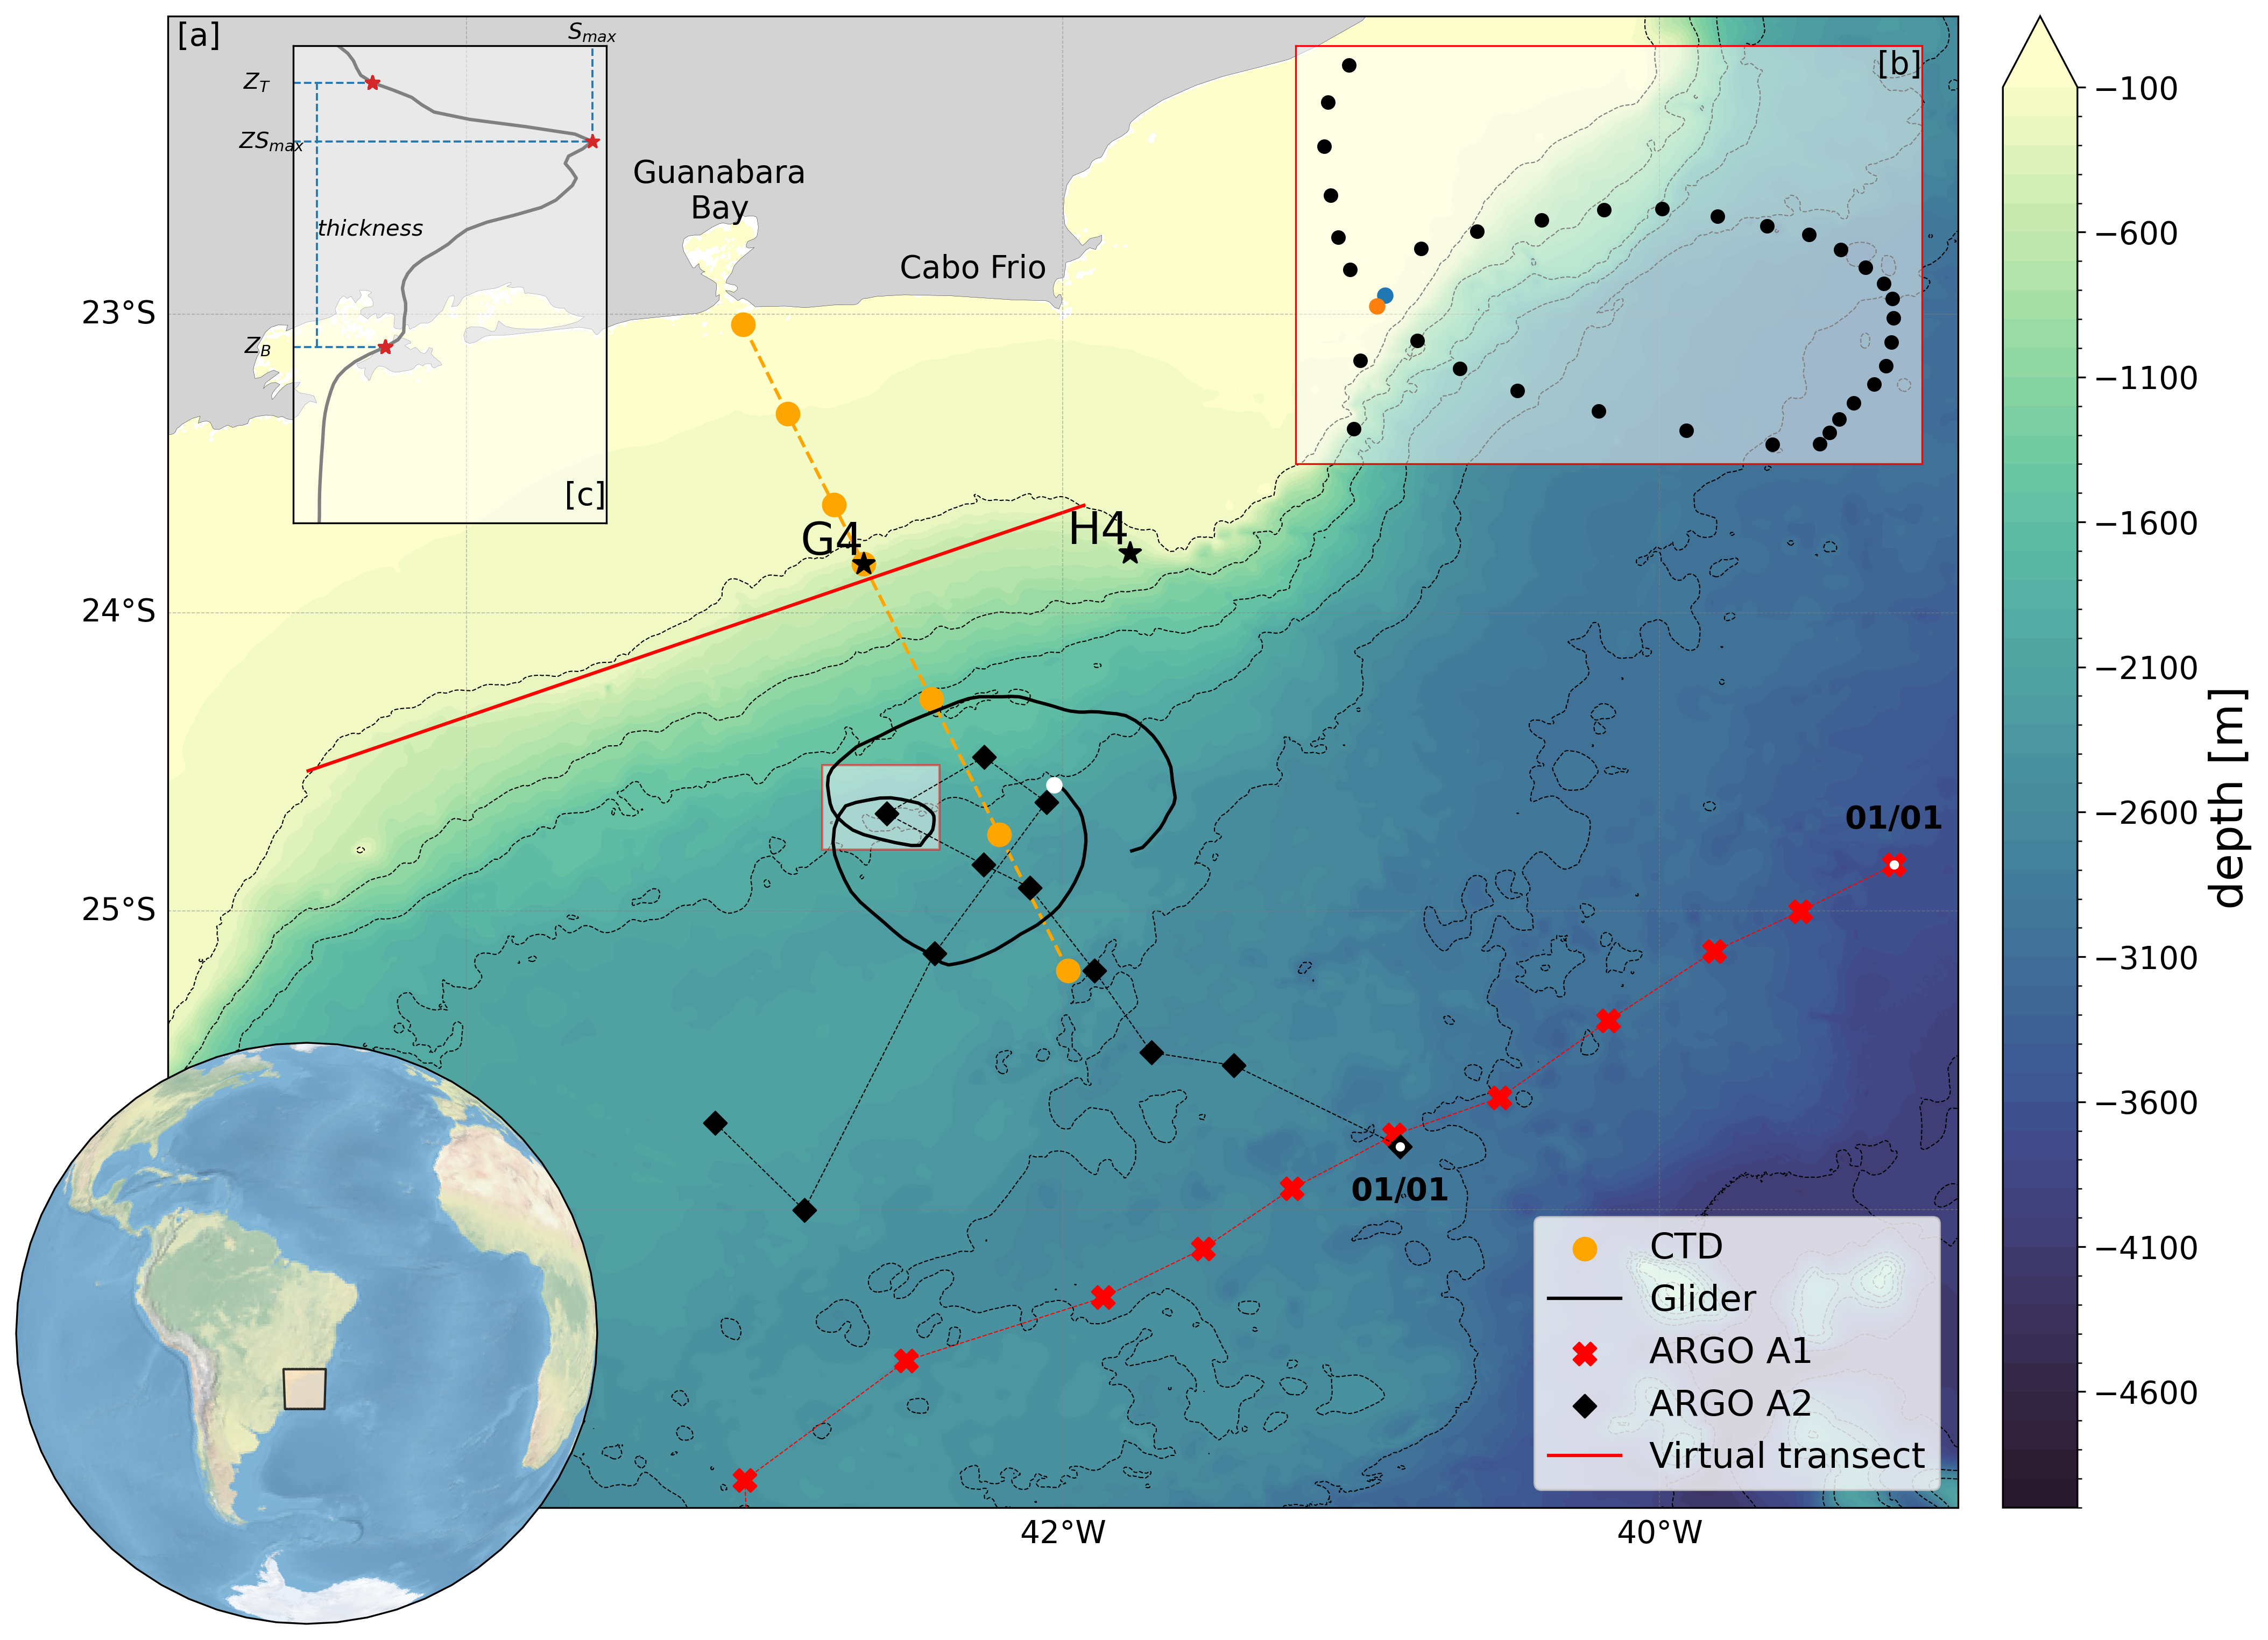
\includegraphics[width=1\linewidth]{figures/00_manuscript_study_area.png}
    \caption{Northeastern South Brazil Bight (NE-SBB) with observational locations in orange representing CTD profiles obtained during the SANAGU2022 cruise; red and black represent ARGO profiles along Line A1 (3901549) and Line A2 (3901225), respectively; the continuous black line represents the Slocum Glider SG19 track; and the red line represents the along-shelf-edge transect used for cross-shelf velocity calculations. The magnified image in the upper right panel highlights a specific part of the glider's path in which a loop was performed. The bathymetric data, marked in color, were extracted from the GEBCO 2019 dataset, and the contours represent the 100-, 200-, 1000-, 2000- and 4000-m isobaths.}
    \label{fig:study_area}
\end{figure}

Thermohaline intrusions may be observed near the bottom, which influence the region by injecting cold and nutrient-rich waters (South Atlantic Central Water, SACW) onto the shelf, thus increasing primary productivity and atmospheric CO$_2$ sequestration \cite{oliveira2019first}. However, recent studies have shown a separate intrusion occurring at mid-depth levels that injects warm and salty waters onto the shelf \cite<Tropical Waters, TW,>{Campos2000,castro2014summer,silva2023inventory}. These intrusions, often called salinity maximum intrusions \cite<hereinafter referred to as $S_{max}$, >{Gordon1981}, sometimes even block the pathway between near bottom nutrient-rich waters and the euphotic zone \cite{silva2023inventory,dottori2023}, thus affecting biogeochemical properties of the shelf and oceanic larval transport \cite{Namiki2017}. These mid-depth salinity maximums, \textit{$S_{max}$}, are generally observed to be associated with the pycnocline \cite{Lentz2003,silva2023inventory} and are responsible for the injection of salt onto the shelf. For instance, in the Middle Atlantic Bight (MAB), \textit{$S_{max}$} drives onshore salt flux, providing half of what is necessary to balance the freshwater input and maintaining the annual average salinity in the region \cite{Gordon1981}. 

Although thermohaline intrusions are linked to a number of mechanisms, such as wind-driven and eddy-driven circulation \cite{Gawarkiewicz1990,GonzalezPola2007,Ruiz2019,Li2012,Malan2020,silver2023increased}, internal waves \cite{Hopkins2012} and baroclinic pressure gradients \cite{Posmentier1978FineFront,Aikman1984}, the drivers of \textit{$S_{max}$} intrusions are still unresolved in the South Brazil Bight (SBB). Considering the dominance of eddies and wind in shaping cross-shelf exchanges \cite{combes2021circulation,calil2021,combes2023circulation}, one might expect that both processes play important roles in developing them. In this study, we investigate the interplay between the geostrophic dynamics of the BC and its eddying meanders and wind-driven circulation and how they might help advect \textit{$S_{max}$} from remote offshore regions all the way to the NE-SBB (Figure~\ref{fig:study_area}). This investigation is motivated by the observation of multiple \textit{$S_{max}$} events advected toward the NE-SBB in March 2022 (Figure~\ref{fig:cruise_transect}), when the last cruises of the Santos Project - Santos Basin Environmental Characterization - coordinated by PETROBRAS \cite{moreira2023multidisciplinary} were conducted. These cruises are named SANAGU2022, which is an acronym for SANtos AGUa and the year of reference.

\begin{figure}[ht!]
    \centering
    \includegraphics[width=0.8\linewidth]{figures/00_manuscript_cruise_transects.png}
    \caption{Transects of absolute salinity (top panels) and temperature (bottom panels), reconstructed using optimum interpolation using CTD profiles obtained during the campaigns SANAGU14 (left) and SANAGU15 (right). The panels presents black isolines related to each property plotted and white isopycnals for 25 $kg\ m^{-3}$ e 25.5 $kg\ m^{-3}$. The x-axis is the horizontal distance from the closest coastline point, while the y-axis is the depth, both in $km$.}
    \label{fig:cruise_transect}
\end{figure}

This study is structured as follows. Section 2 describes the dataset used and methods applied. Section 3 presents our results and shows preferential \textit{$S_{max}$} pathways of advection. Section 4 discusses the interaction between BC dynamics and wind and presents a set of Lagrangian simulations to aid in interpreting the advective pathways. Finally, Section 5 highlights the major conclusions of this study.

\section{Material and Methods}
\label{section:methods}

\subsection{Hydrographic Dataset}
In this study, we use a diverse set of data from several sources, including in situ measurements, remotely sensed products and global numerical reanalysis (as summarized in Table~\ref{tab:dataset}). 

The SANAGU2022 cruise was carried out during March 2022, sampling the entire South Brazil Bight, as described in \citeA{moreira2023multidisciplinary}. Only transects over the NE-SBB were initially investigated (Figure~\ref{fig:study_area} thin orange lines). For this particular work, we considered only the central transect, off Guanabara Bay (Figure~\ref{fig:study_area} orange markers), since intrusions were only observed along this transect. The transect was sampled twice within 2 weeks: the first sampling took place from 5 to 14 March and second was performed between 23 to 28 March.The CTD profiles were taken using a SBE 911 Plus equipment, with stations aligned almost perpendicular to the coastline (Figure~\ref{fig:study_area} an orange dashed line). We highlight that only the central transect is used in this manuscript, since intrusions were only observed in this one. Quality control and processing methods were applied using a modified version of the Python-CTD package \cite{Fernandes2014,dottori2023}. In the processing workflow, we removed spikes, averaged the data into 1 $m$ bin and applied a 7-point (21-point) window Hanning filter to smooth the profiles over the shelf (slope). This processing is similar to the one applied by \citeA{silva2023inventory} and \citeA{dottori2023} over the same continental shelf and by \citeA{silveira2023} for the slope casts.

\begin{table}
\caption{Summary of observational dataset used in this work, along with its source (name or reference), extracted variables and period of analysis.}
\centering
\begin{tabular}{l c c c}
\hline
 \textbf{dataset} & \textbf{source} & \textbf{variables} & \textbf{period} \\
\hline
        CTD           & - & T,S & Mar, 2023 \\ 
        ARGO          & ARGO & T,S & Jan-Mar, 2023 \\ 
        Glider        & ProjetoAzul & T,S & Feb-Mar, 2023 \\ 
        AVISO         & CMEMS & Gridded Altimetry & Jan-Mar, 2023 \\ 
        AVISO         & CMEMS & Along track altimetry & Jan-Mar, 2023 \\ 
        ERA5          & \cite{hersbach2018era5} & Wind stress & Jan-Mar, 2023 \\ 
        GLORYS12V1    & CMEMS & u,v,T,S & Jan-Mar, 2023 \\ 
        MERGE         & \cite{rozante2010combining} & Precipitation & Jan-Mar, 2023 \\ 
        AVHRR         & - & SST & Jan-Mar, 2023 \\ 
        META3.1exp DT & \cite{pegliasco2022} & Eddie track & Jan-Mar, 2023 \\ 
\hline
\end{tabular}
\end{table}

ARGO profiles were taken using the argopy python toolbox \cite{Maze2020}, fetched from the \textit{Institut Français de Recherche pour l’Exploitation de la Mer} (IFREMER) server in April 2023 (Figure~\ref{fig:study_area}, back and red markers). The temporal and spatial filtering of the dataset resulted in two profilers: 3901549 and 3901225, defined hereafter as A1 and A2, respectively. From these instruments, we extracted profiles with a quality flag of 1 or 2, indicating "good data" or "probably good data", which means reprocessed profiles \cite{notarstefano2020argo}. The Glider dataset was obtained at the ProjetoAzul portal (\url{http://www.projetoazul.eco.br/}, accessed in May 2023). The metadata available within the dataset presents quality control flags, suggesting that the dataset was pre processed before sharing (Figure~\ref{fig:study_area}). We only use information with quality flag 0, which means "good data". Hydrographic properties, such as absolute salinity and potential density, from all vertical profiles available were derived from in situ measurements, using the TEOS-10 toolbox \cite{mcdougall2011gsw} through the GSW python package \cite{firing2021gsw}. 

\subsection{Characteristics of Salinity Maximum intrusions}
\label{sec:smax_structure}

In this work, we used the intrusion characteristics presented by \citeA{silva2023inventory}, which was created by adapting the detection algorithm from \citeA{Lentz2003} for the SBB thermodynamics. These characteristics are illustrated in Figure~\ref{fig:smax}, using an observed absolute salinity vertical profile. The maximum salinity identified is defined as \textit{$S_{max}$} and its corresponding vertical position is $ZS_{max}$. However, the profile is only defined as intrusion if the vertical gradient ($\Delta{S}$) exceeds a threshold (here we used $0.1 g\ kg^{-1}$ following \citeA{silva2023inventory}. Once an intrusion is identified, the extraction of its properties is done by finding their thickness, defined as the difference between the top ($Z_{T}$) and bottom ($Z_{B}$) boundaries. These limits are given based on the depth in which the difference between the salinity peak decreases in 75$\%$ relative to the surface minimum salinity. Note that identifying the boundaries of an intrusion differs significantly from the original algorithm of \citeA{Lentz2003}, because salinity is supposed to increase in the region where this method was developed, while in the SBB salinity increases and then decreases, based on the local water mass distribution. Further description on these adaptations are given in \citeA{silva2023inventory}. We highlight that this same adapted algorithm was used in this work, to identify intrusions within the dataset. 

\begin{figure}[ht!]
    \centering
    \includegraphics[width=0.5\linewidth]{figures/00_manuscript_smax_schematic.png}
    \caption{Sample absolute salinity profile showing the salinity maximum (\textit{$S_{max}$}) characteristics: $ZS_{max}$ is the depth of the \textit{$S_{max}$}; $Z_{T}$ and $Z_{B}$ are the depths of the top and bottom boundaries, respectively; and $thickness$ is the difference between them. The \textit{$S_{max}$} characteristics were extracted based on the adaptations of the \protect\citeA{Lentz2003} algorithm of \protect\citeA{silva2023inventory}.}
    \label{fig:smax}
\end{figure}

\subsection{Altimeter Dataset}
To complement our comprehensive analysis, we retrieved the sea surface elevation and geostrophic velocities derived from a global altimeter product, available by the Copernicus Marine Environment Monitoring Service (CMEMS). Here, we used both L4 gridded (\url{https://doi.org/10.48670/moi-00149}, accessed in April 2023) products as well as the L2 along track altimeter data (\url{https://doi.org/10.48670/moi-00146}, accessed in April 2023) to reconstruct the mesoscale scenarios. The gridded sea level anomaly (SLA) product has a 0.25$^o$ spatial resolution at daily frequency and it merges data from all available altimeter missions, applying an optimal interpolation to construct the final product. Those products were processed by SSALTO/DUACS and distributed by AVISO+ (\url{https://www.aviso.altimetry.fr}) with support from CNES. Using geostrophy for the gridded SLA field, we obtained the zonal and meridional geostrophic currents using Equations~\ref{eq:geostrophic_a} and~\ref{eq:geostrophic_b}.  To visualize the mesoscale features with better resolution, we used the along track altimeter to compute the geostrophic velocity normal to the track. This technique provides velocities with an average resolution of 7 $km$ which vary among satellites and was recently applied to investigate the Gulf Stream dynamics and its relation with Salinity Maximum intrusions in this region \cite{silver2023increased}. Among the satellite data available during the period and within the region, we selected tracks which crossed the features of interest, such as the Brazil Current and the eddy dipoles present during February and March of 2022. It resulted in a total of 19 tracks (see Figure~\ref{fig:geostrophic_fields}). The cross-track velocities ($U_{ct}$) were obtained from the along-track SLA fields (from high resolution track data) by using \ref{eq:geostrophic_c}. These cross-track velocities are also shown along the tracks in Figure~\ref{fig:geostrophic_fields}. 

%  Numbered lines in equations:
%  To add line numbers to lines in equations,
\begin{linenomath*}

\begin{equation}
\label{eq:geostrophic_a}
U_{g}  = - \frac{g}{f} \frac{\Delta{SLA}}{\Delta x} {\textit{(- gridded SLA)}}
\end{equation}

\begin{equation}
\label{eq:geostrophic_b}
V_{g}  = \frac{g}{f} \frac{\Delta{SLA}}{\Delta y} {\textit{(- gridded SLA)}}
\end{equation}

\begin{equation}
\label{eq:geostrophic_c}
U_{ct}  = - \frac{g}{f} \frac{\Delta{SLA}}{\Delta s} {\textit{(- track SLA)}}
\end{equation}
\end{linenomath*}

where, $g$ is the gravity acceleration, $f$ is the Coriolis parameter computed with the TEOS 10 GSW \cite{mcdougall2011gsw} and '$\Delta s$' is the along-track grid resolution ($\approx 7 km$).

In addition to the geostrophic fields, we also used the altimetric Mesoscale Eddy Trajectories Atlas multi-satellite delayed-time product \cite<META3.1exp,>{pegliasco2022}, to explore the eddy activity during the period. The Mesoscale Eddy Trajectory Atlas products were produced by SSALTO/DUACS and distributed by AVISO+ (\url{https://www.aviso.altimetry.fr/}). This dataset provides the eddy position, speed, amplitude and other information about eddies, detected with the py-eddy-tracker algorithm \cite{mason2014new} applied over the absolute dynamic topography (ADT) from the gridded AVISO product. This dataset was filtered to select cyclones and anticyclones from January to March, 2022, over the domain of interest.

\subsection{Other Dataset}
To provide a context on the meteo-oceanographic conditions, several datasets were used to complement the ones described in previous sections. The satellite sea surface temperature (SST) were obtained from the Advanced Very High Resolution Radiometer (AVHRR) Level 3 dataset, with a 4-km resolution at daily frequency \cite<\url{https://www.ncei.noaa.gov/products/avhrr-pathfinder-sst}, >{saha2018avhrr}. Precipitation was retrieved from the MERGE dataset \cite<\url{http://ftp.cptec.inpe.br/modelos/tempo/MERGE/GPM/DAILY/}, >{rozante2010combining}, which combines satellite precipitation data from the Tropical Rainfall Measuring Mission (TRMM) with surface observations from meteorological stations over the South American continent. This product results in maps of daily accumulated precipitation with a 12-km spatial resolution. The meteorological conditions were also analyzed using hourly wind stress at the surface, retrieved from the fifth generation reanalysis (ERA5, \url{https://doi.org/10.24381/cds.adbb2d47}), provided by the European Centre for Medium-range Weather Forecasts (ECMWF). This dataset has a 0.25$^o$ resolution and combines data from satellites, buoys and meteorological stations \cite{hersbach2018era5}. From these three dataset, we extracted information from January to March, 2022.

\subsection{Dynamical computations}

\subsubsection{Cross-shelf edge exchanges}
To identify the cross-shelf surface response to winds during January and March 2022, we computed the Ekman Transport using wind stress \cite<Equation~\ref{eq:ekman}, >{brink2016,gangopadhyay2022introduction}: 

\begin{linenomath*}
\begin{eqnarray}
    \label{eq:ekman}
    T_{Uek}  & = & \frac{\tau^{ERA5}_y}{f \rho} H \nonumber \\
    T_{Vek} & = & - \frac{\tau^{ERA5}_x}{f \rho} H
\end{eqnarray}
\end{linenomath*}

where $T_{Uek}$ and $T_{Vek}$ is the zonal and meridional Ekman transport, $\tau_{x}$ and $\tau_{y}$ the zonal and meridional wind stress components, $H = 30\ m$ is the approximate mixed layer depth computed from the hydrographic dataset, $\rho = 1028 kg\ m^{-3}$ is the water density. 

We used wind stress from the ERA5 dataset then rotated the transport using the average shelf break orientation, to estimate the wind-driven cross-shelf exchange over the shelf break. Here, we considered the 200-m isobath as the reference for the shelf break and extracted the isobath location from the GEBCO dataset \cite{weatherall2015new}. To identify hotspots in which the cross-shelf geostrophic velocity supports onshore transport, we also applied this same methodology for the geostrophic gridded fields from the AVISO dataset. We selected velocity vectors over the shelf break and rotated them using the same approach as in the Ekman Transport. In both rotated velocities, positive (negative) values indicates offshore (onshore) flows in the cross-shelf direction and northeastward (southwestward) in the alongshelf direction (see Figure~\ref{fig:study_area}, top-left inset).

\subsubsection{Other calculations}
Considering that \textit{$S_{max}$} intrusions correlates with the maximum stratification in a water column, and thus are found associated with the pycnocline \cite{silva2023inventory}, it is helpful to calculate the mixed layer depth (MLD), to investigate if the intrusion signals are consistent with the common features in the region. The MLD was found through the implementation of the gradient density criteria \cite{lorbacher2006ocean}, with a  threshold of 0.025 $kg\ m^{-3}$.  We chose this criteria to account for stratification influenced by both temperature and salinity. This is relevant as  the temperature criteria \cite<e.g.,>{de2004mixed} may not be representative of MLD where salinity gradients are important, such as in the SBB \cite{silveira2023,sasaki2024}. 

To understand the response of cross-shelf circulation to upwelling favorable winds at the shelf break, we computed the Burger number (\ref{eq:burger}):

\begin{linenomath*}
\begin{equation}
\label{eq:burger}
Bu = \frac{N*\alpha}{f}
\end{equation}
\end{linenomath*}

where $N$ is the Brunt-Vaisalla frequency, computed using the GSW python package \cite{firing2021gsw}, and $\alpha$ is the topographic gradient ($\alpha = \frac{dh}{dx'}$, where $x'$ is the cross-isobath direction), extracted from the GEBCO bathymetric dataset in the nearest locations to the CTD casts used. With this nondimensional number, it is possible to address if there will be a baroclinic ($Bu \geq 1$) or barotropic ($Bu < 1$) response \cite{clarke1985,LentzChapman2004}. This is important because in the first case, the onshore current opposite to the upwelling-favorable wind-driven circulation will take place in mid-waters, above the bottom layer \cite{LentzChapman2004}. 

\subsection{Lagrangian experiments}
Offline lagrangian experiments were conducted to assess the probable pathways leading to the \textit{$S_{max}$} observed over the SBB. We chose the OceanParcels v2.4 model \cite{delandmeter2019parcels} to perform these experiments, due to its wide applications in the literature to understand trajectories in  the ocean using general ocean circulation model outputs \cite{valles2022water,dawson2023pathways,seijo2023intrusions}. The advection of virtual particles employs a fourth-order Runge-Kutta iteration scheme \cite{delandmeter2019parcels}, using velocity fields from the GLORYS12V1 global reanalysis (\url{https://doi.org/10.48670/moi-00016}). This product provides daily hydrodynamic fields, in a 0.08$^o$ horizontal resolution, assimilating a large observational dataset. The experiment setup uses an extra module that delete particles that reaches any closed boundary, that way avoiding accumulation at the boundaries. The Table~\ref{tab:lagrangian_experiments} summarizes the lagrangian experiments and the differences, which were selected based on the \textit{$S_{max}$} observations. They are explained in Section~\ref{subsec:setup}.

\begin{table}[ht!]
\label{tab:lagrangian_experiments}
\caption{Summary of lagrangian analysis performed, along with the hydrodynamical fields used as source information, the seeding depth of release for 3D experiments and which mode were run (B for back propagation and F for forward propagation).}
\begin{tabular}{c c c c}
\hline
\textbf{experiment} & \textbf{hydrodynamical field [u,v]} & \textbf{seeding depth [m]} & \textbf{mode {[}B/F{]}} \\
\hline
BI                  & GLORYS 3D                     & 50                     & B                       \\ 
BII                 & GLORYS 2D ISOPYCNAL           & -                      & B                       \\ 
BII                 & GEOSTROPHIC                   & -                      & B                       \\ 
FNI                 & GLORYS 3D                     & 75                     & F                       \\ 
FNII                & GLORYS 2D ISOPYCNAL           & -                      & F                       \\ 
FNIII               & GEOSTROPHIC                   & -                      & F                       \\ 
FEI                 & GLORYS 3D                     & 75                     & F                       \\ 
FEII                & GLORYS 2D ISOPYCNAL           & -                      & F                       \\ 
FEIII               & GEOSTROPHIC                   & -                      & F                       \\ 
\hline
% \multicolumn{2}{l}{$^{a}$Footnote text here.}
\end{tabular}
\end{table}

\section{Results}
\label{section:description}

\subsection{Salinity Maximum intrusions during March 2022}
\label{subsec:smaxdesc}

Hydrographic transects reveal differences in the oceanographic conditions during the SANAGU14 and SANAGU15 cruises, within a 2-weeks span, at the Northeastern region of the South Brazil Bight (NE-SBB). The first transect (Figure~\ref{fig:cruise_transect} a,b) presents larger differences of temperature along the transect. Near the bottom, waters colder than 18$^o$C indicate the presence of the cold and nutrient-rich South Atlantic Central Water (SACW). This water mass is found throughout the year in that area under northeasterly wind conditions, as response to the offshore surface Ekman Transport \cite{cerda2014,castro2014summer,dottori2023}. The onshore advection also tilts isopycnals positively towards the coast (Figure~\ref{fig:cruise_transect} a,b). From the shelf edge to offshore (the shelf-sea interface), water warmer than 25ºC with salinity higher than 36  $g\ kg^{-1}$ were found, indicating the presence of Tropical Water (TW) \cite{cerda2014,castro2014summer}. It is interesting, however, to notice the presence of a well-defined \textit{$S_{max}$} intrusion at 25 $km$ from the coast and at 20 $m$ depth (first week, Figure~\ref{fig:cruise_transect} a). This intrusion has a thickness of approximately 20 $m$, with associated waters saltier than 36 $g\ kg^{-1}$. A second signal is observed over the shelf edge, between 25 and 50 $m$ depth, corresponding to an \textit{$S_{max}$} intrusion of 25 $m$ thick, but saltier than the other one (S > 37 $g\ kg^{-1}$), and it is crossing the isopycnals (white dashed lines in Figure~\ref{fig:cruise_transect}).

\begin{figure}[ht!]
    \centering
    \includegraphics[width=0.8\linewidth]{figures/00_manuscript_cruise_transects.png}
    \caption{Transects of absolute salinity (top panels) and temperature (bottom panels), reconstructed using optimum interpolation using CTD profiles obtained during the campaigns SANAGU14 (left) and SANAGU15 (right). The panels presents black isolines related to each property plotted and white isopycnals for 25 $kg\ m^{-3}$ e 25.5 $kg\ m^{-3}$. The x-axis is the horizontal distance from the closest coastline point, while the y-axis is the depth, both in $km$.}
    \label{fig:cruise_transect}
\end{figure}

Two weeks later, the second transect (Figure~\ref{fig:cruise_transect} c,d) reveals different hydrographic conditions. Over the shelf, the coldest waters are higher than 18$^o$C and isopycnals are flatter than before, suggesting a possible shutdown in the cold and nutrient-rich water advection towards the coast. However, this transect shows the presence of two \textit{$S_{max}$} regions coming on to the shelf, with similar characteristics as the one from the first transect. The \textit{$S_{max}$} over the shelf edge is observed above the 25 $kg\ m^{-3}$ isopycnal, while the second one, much offshore, is observed below this isopycnal. Over the inner shelf, the intrusion advanced about 10 $km$ towards the coast, but became thinner (10 $m$). 

Remotely sensed Sea Surface Temperature (SST) shows a 4$^o$C cross-shelf gradient, with waters colder than 22$^o$C on the shelf and warmer than 26$^o$C offshore, during SANAGU14 (Figure S1 a). This horizontal gradient is suggestive of cold water uplift in response to upwelling-favorable northeasterly winds \cite{emilsson1961shelf,dottori2023}. During the second transect (Figure S1 b), the cross-shelf gradient is relatively weaker (~2 $^o$C). These changes are consistent with the long transect surface layers changes observed during the cruises (Figure~\ref{fig:cruise_transect} a and c).

The weather conditions during both transects were different, which in turn may be responsible for the differences in the SST conditions. During the first cruise, it was observed a low precipitation, therefore weaker cloud coverage, and the presence of upwelling-favorable winds (Figure S2 a). These conditions reduced the shelf temperatures, while increasing the offshore SST, contributing to the relatively larger gradient observed. During the second cruise, however, the passage of a frontal system a few days prior to the observations, contributed to reduce the SST gradient throughout the domain, by increasing the cloud coverage and also weakening the Ekman transport due to reduction of wind intensity (Figure S2 c).

The mesoscale footprints are observed in remotely sensed images associated with the presence of \textit{$S_{max}$} during the period. For instance, it is noteworthy the CFE signal in the SST, during both cruises (Figure S1), offshore the NE-SBB (centered in, approximately, 25$^o$S and 42$^o$W). In addition, since this region is highly dynamic due to the baroclinic instability associated to the Brazil Current system and its meanders \cite{silveira2008,uchoa2023}, it is useful to investigate the mesoscale dynamics during the period. From the geostrophic currents (Figure~\ref{fig:geostrophic_fields}), the CFE is present from February to March, centered at approximately 24.5$^o$S and 41.5$^o$W. During February, the CFE associated velocities are up to 0.5 $m.s^{-1}$, and it loses strength in March, presenting velocities of 0.4 $m\ s^{-1}$. Nevertheless, its influence over the SST field is depicted in Figure S1 a and b, at the same location, mainly by a cold water tongue at the eastern edge of the eddy. At the end of March, it appears the BC splits in two branches at 24$^o$S and 41.5$^o$W, with one branch flowing along the shelf edge, westward, and another branch flowing southwestward. This second branch meanders around a weaker CFE, and then attaches back to the shelf edge near 24$^o$S and 42.3$^o$W. The meander influence on cross-shelf currents is clearly observed considering an along-shelf edge cross-shelf geostophic current Hovmoller (Figure S3 a). This analysis shows two centers of shoreward currents more intense than two standard deviation from the historical average (1992-2022, Figure S3 b). The projected shoreward geostrophic current occur between 24.5$^o$S and 24.0$^o$S, the same spot where the BC meander attaches back to the shelf edge. Therefore, it is expected that mesoscale activity plays an important role over the cross-shelf exchanges, in addition to upwelling-favorable winds response.

\begin{figure}[ht!]
    \centering
    \includegraphics[width=0.8\linewidth]{figures/00_manuscript_geostrophic_fields.png}
    \caption{Sea surface elevation anomalies (in colors), from gridded AVISO for (a) 16th February, (b) 21st February, (c) 7th March and (d) 27th March. Geostrophic fields overlaid the plots in gray vectors, for gridded AVISO, and computed using along-track altimeter information in black vectors. Green markers represents locations of CTD profiles obtained by the time of the each plot and red markers are the locations of the ARGO profiles.}
    \label{fig:geostrophic_fields}
\end{figure}

\subsection{Cross-shelf connectivity}
\label{subsec:cross}
In the previous section, we presented the hydrographic observations made during the cruises, which revealed the presence of \textit{$S_{max}$} intrusions (Figure~\ref{fig:cruise_transect}). One might question the origin of these structures and how they entered the continental shelf. To address these questions, we investigated the water mass characteristics and their advective velocities in this region using available ARGO profiles, a Glider dataset, and altimeter (both gridded fields and tracks) in the weeks leading to and during the cruise. We describe the results using the ARGO observations and Glider data to establish a plausible pathway indicating cross-shelf connectivity in this subsection. The two available ARGO paths chosen are shown by lines A1 (February) and A2 (February-March) in Figure~\ref{fig:study_area}. 

In the prior weeks to the cruises, we identified \textit{$S_{max}$} signals from deep waters to the shelf edge, from different measurement platforms, which may have potential connections to the intrusions observed over the shelf. 
\textit{$S_{max}$} signals were observed in two ARGO profilers, showing consistency in their properties. In both datasets, the \textit{$S_{max}$} exhibited absolute salinity values exceeding 37.1 $g\ kg^{-1}$ at its core, with an increase of approximately 0.3 $g\ kg^{-1}$ from the surface. These signals were detected at depths ranging from 50 to 75 $m$, situated below the mixed layer and between the 25 and 25.5 $kg\ m^{-3}$ isopycnals (Figure~\ref{fig:argo_alongshelf} and Figure~\ref{fig:argo_crossshelf}). However, there was a temporal mismatch in the observation of \textit{$S_{max}$} between the ARGO profiles. The first ARGO (A1) recorded \textit{$S_{max}$} between January 20$^{th}$ and February 1$^{st}$, while during the same period, the second ARGO (A2) did not show any intrusion signal (Figure~\ref{fig:argo_alongshelf} and Figure~\ref{fig:argo_crossshelf}). Nevertheless, later on, the \textit{$S_{max}$} signal was observed from February 15$^{th}$ to the end of March, as the ARGO drifted closer to the shelf edge. The similarities between these observations, particularly in the vertical position, suggest that we are observing the same feature. According to the ARGO tracks, this signal is moving toward the shelf edge, observed 50 and 40 days, respectively, prior to the \textit{$S_{max}$} observation over the shelf. Although ARGO observations were highly valuable, their southwesterly drift does not allow a further analysis.

\begin{figure}[ht!]
    \centering
    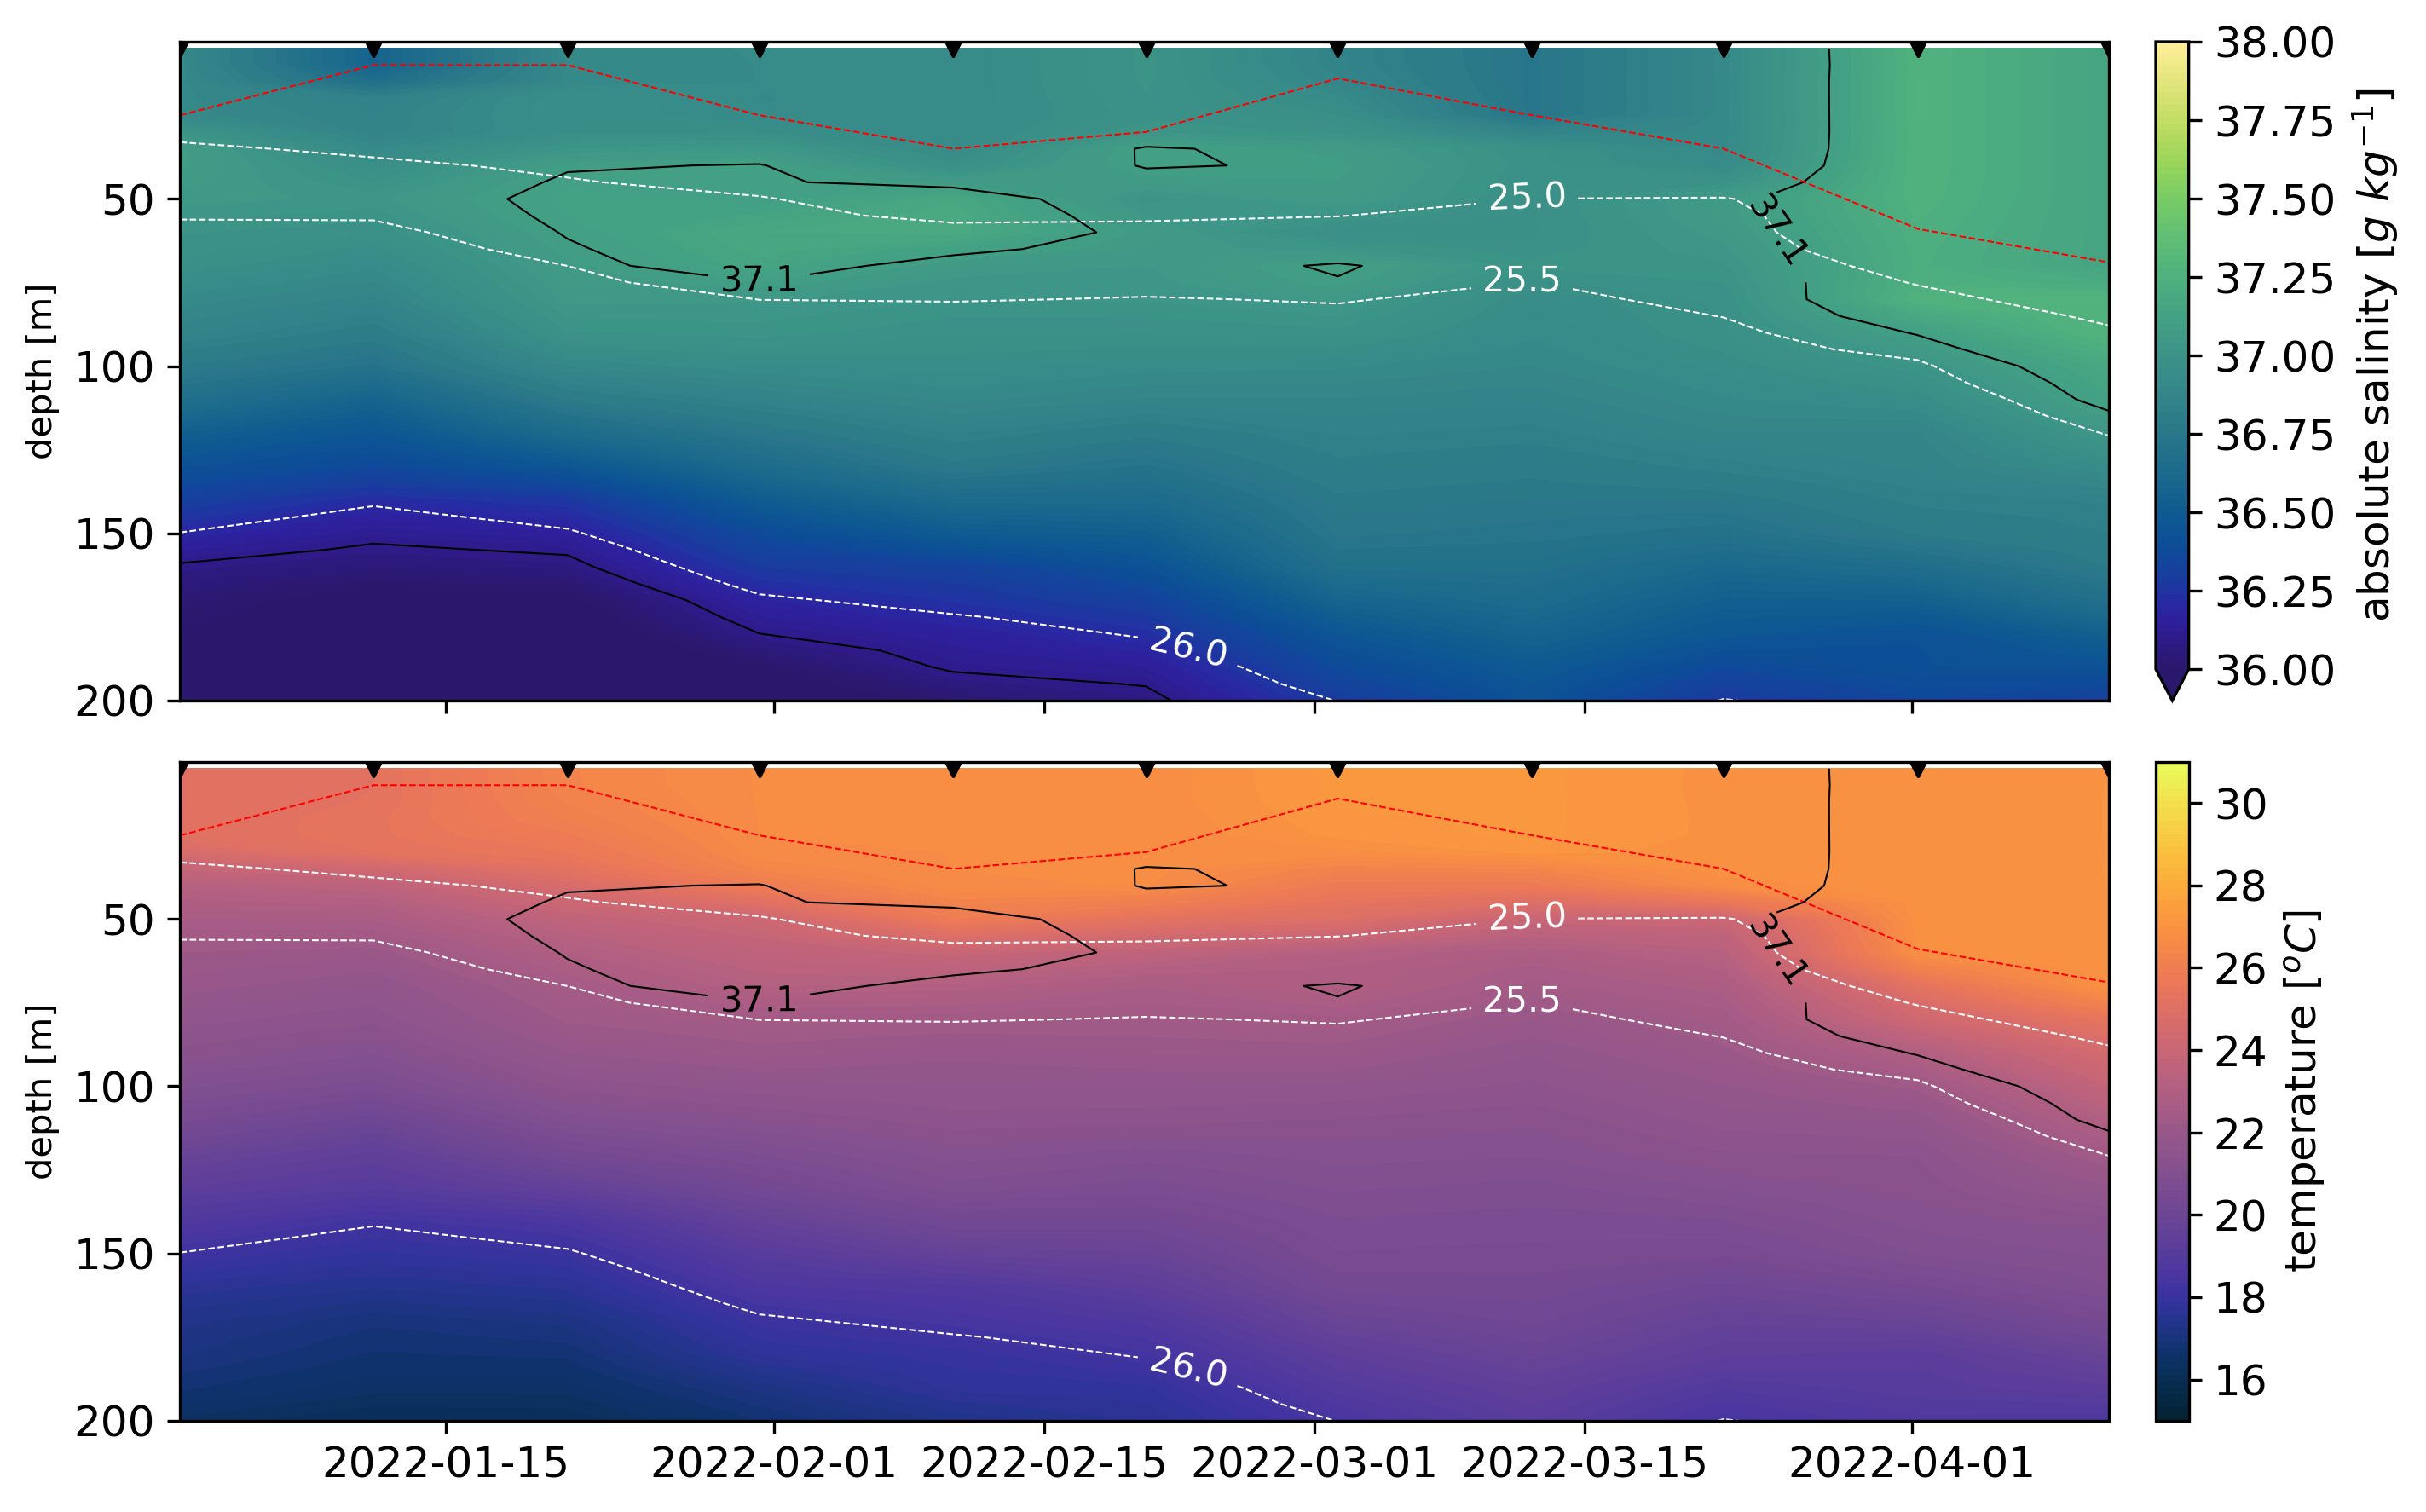
\includegraphics[width=0.8\linewidth]{figures/00_manuscript_argo_alongshelf.png}
    \caption{Transects reconstructed from ARGO profiles along line A1 in Figure~\ref{fig:study_area}  (WMO ID 3901549), for absolute salinity (top panel) and temperature (bottom panel). The black line indicates the 37.1 $g\ kg^{-1}$ isohaline, the white isopycnals for 25, 25.5 and 26 $kg\ m^{-3}$ and red dashed lines indicate the mixed layer depth, using the density criteria. The x-axis is time, while the y-axis is the depth in $m$. The path of the float is shown from east (right) to west (left) in \protect Figure~\ref{fig:study_area} as red markers}.
    \label{fig:argo_alongshelf}
\end{figure}

\begin{figure}[ht!]
    \centering
    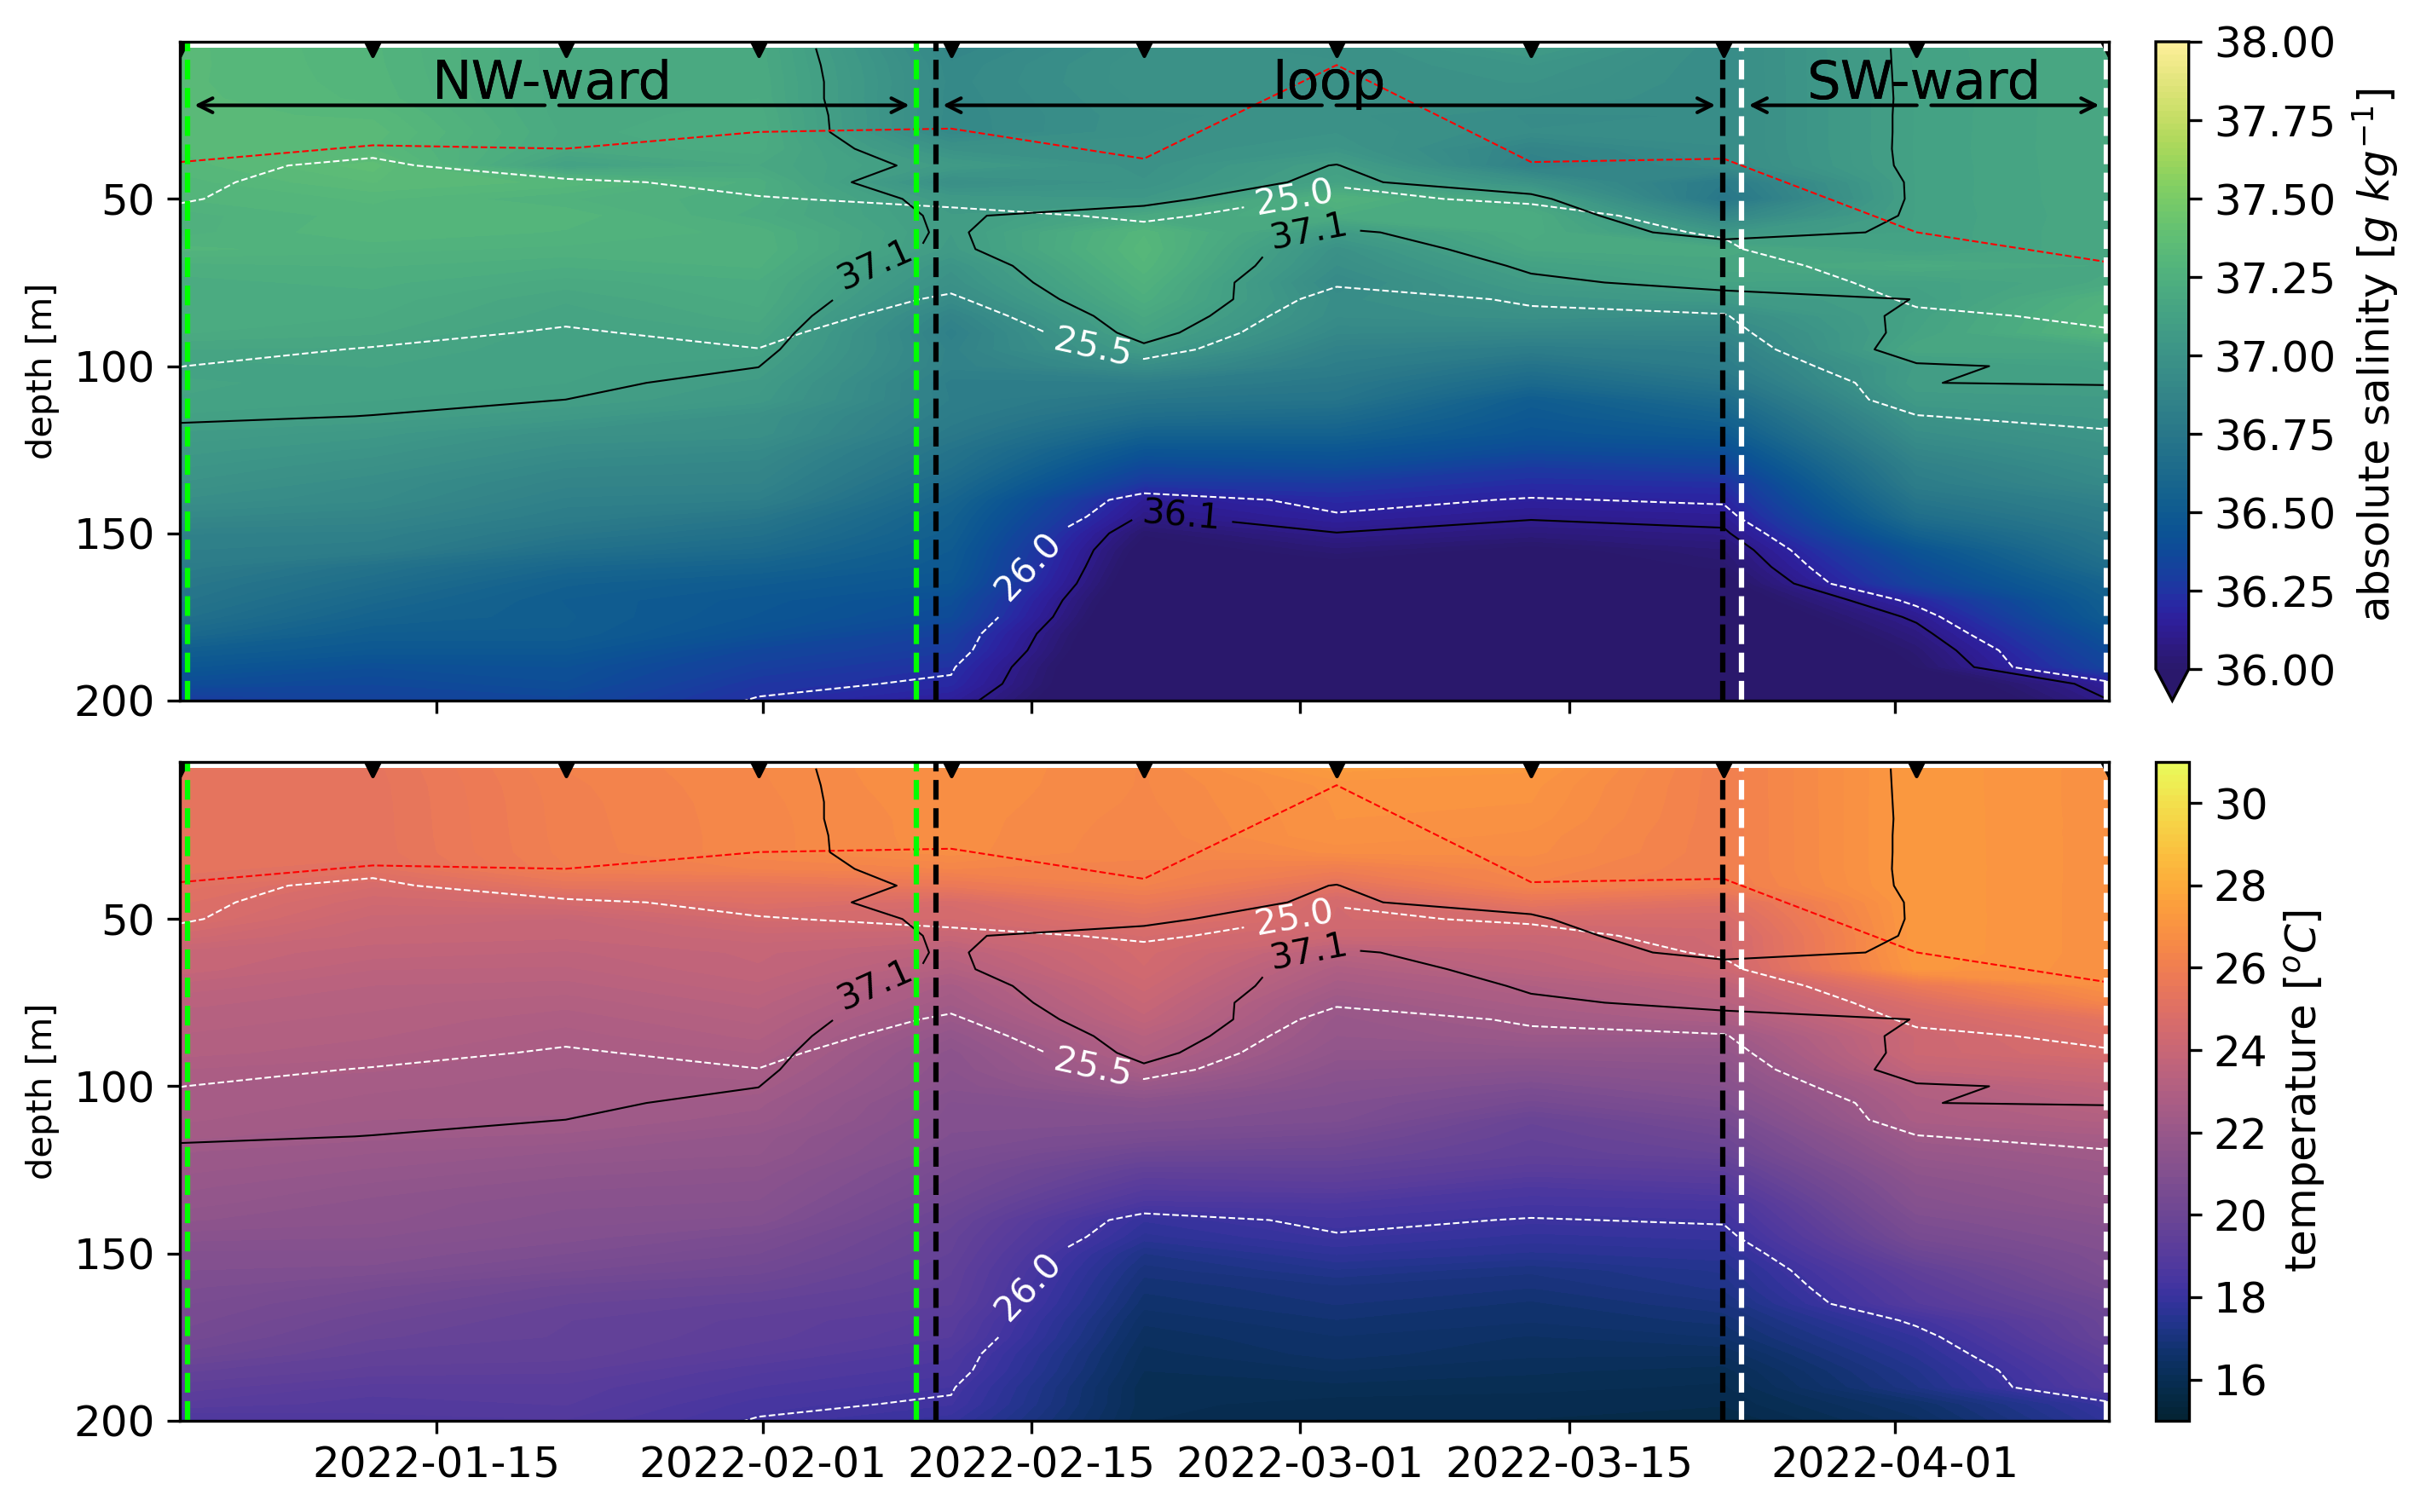
\includegraphics[width=0.8\linewidth]{figures/00_manuscript_argo_crossshelf.png}
    \caption{Same as Figure~\ref{fig:argo_alongshelf}, but for ARGO along line A2 in Figure~\ref{fig:study_area} (WMO ID 3901225) and its path from South (left) to North (right) is found in \protect Figure~\ref{fig:study_area} as black markers.}
    \label{fig:argo_crossshelf}
\end{figure}

The Slocum Glider (SG19) sampled this region during March 2022 and enabled the examination of the \textit{$S_{max}$} advection towards the shelf edge. In this dataset, intrusion signals were observed (Figure~\ref{fig:glider_transect}), with similar properties than the ones observed in the previous dataset. To describe the hydrography from the glider (Figure~\ref{fig:glider_transect}), we divided the glider trajectory in three segments for analysis: the first, and with most offshore observations, extends from March 3$^{rd}$ to 12$^{th}$ (Figure~\ref{fig:glider_transect} a), the second is the loop pattern described by the glider (Figure~\ref{fig:glider_transect} b) and it goes from 13$^{th}$ to 19$^{th}$ March and the last half is the most onshore observations (Figure~\ref{fig:glider_transect} c) with data from 22$^{th}$ to 27$^{th}$ March.

\begin{figure}[ht!]
    \centering
    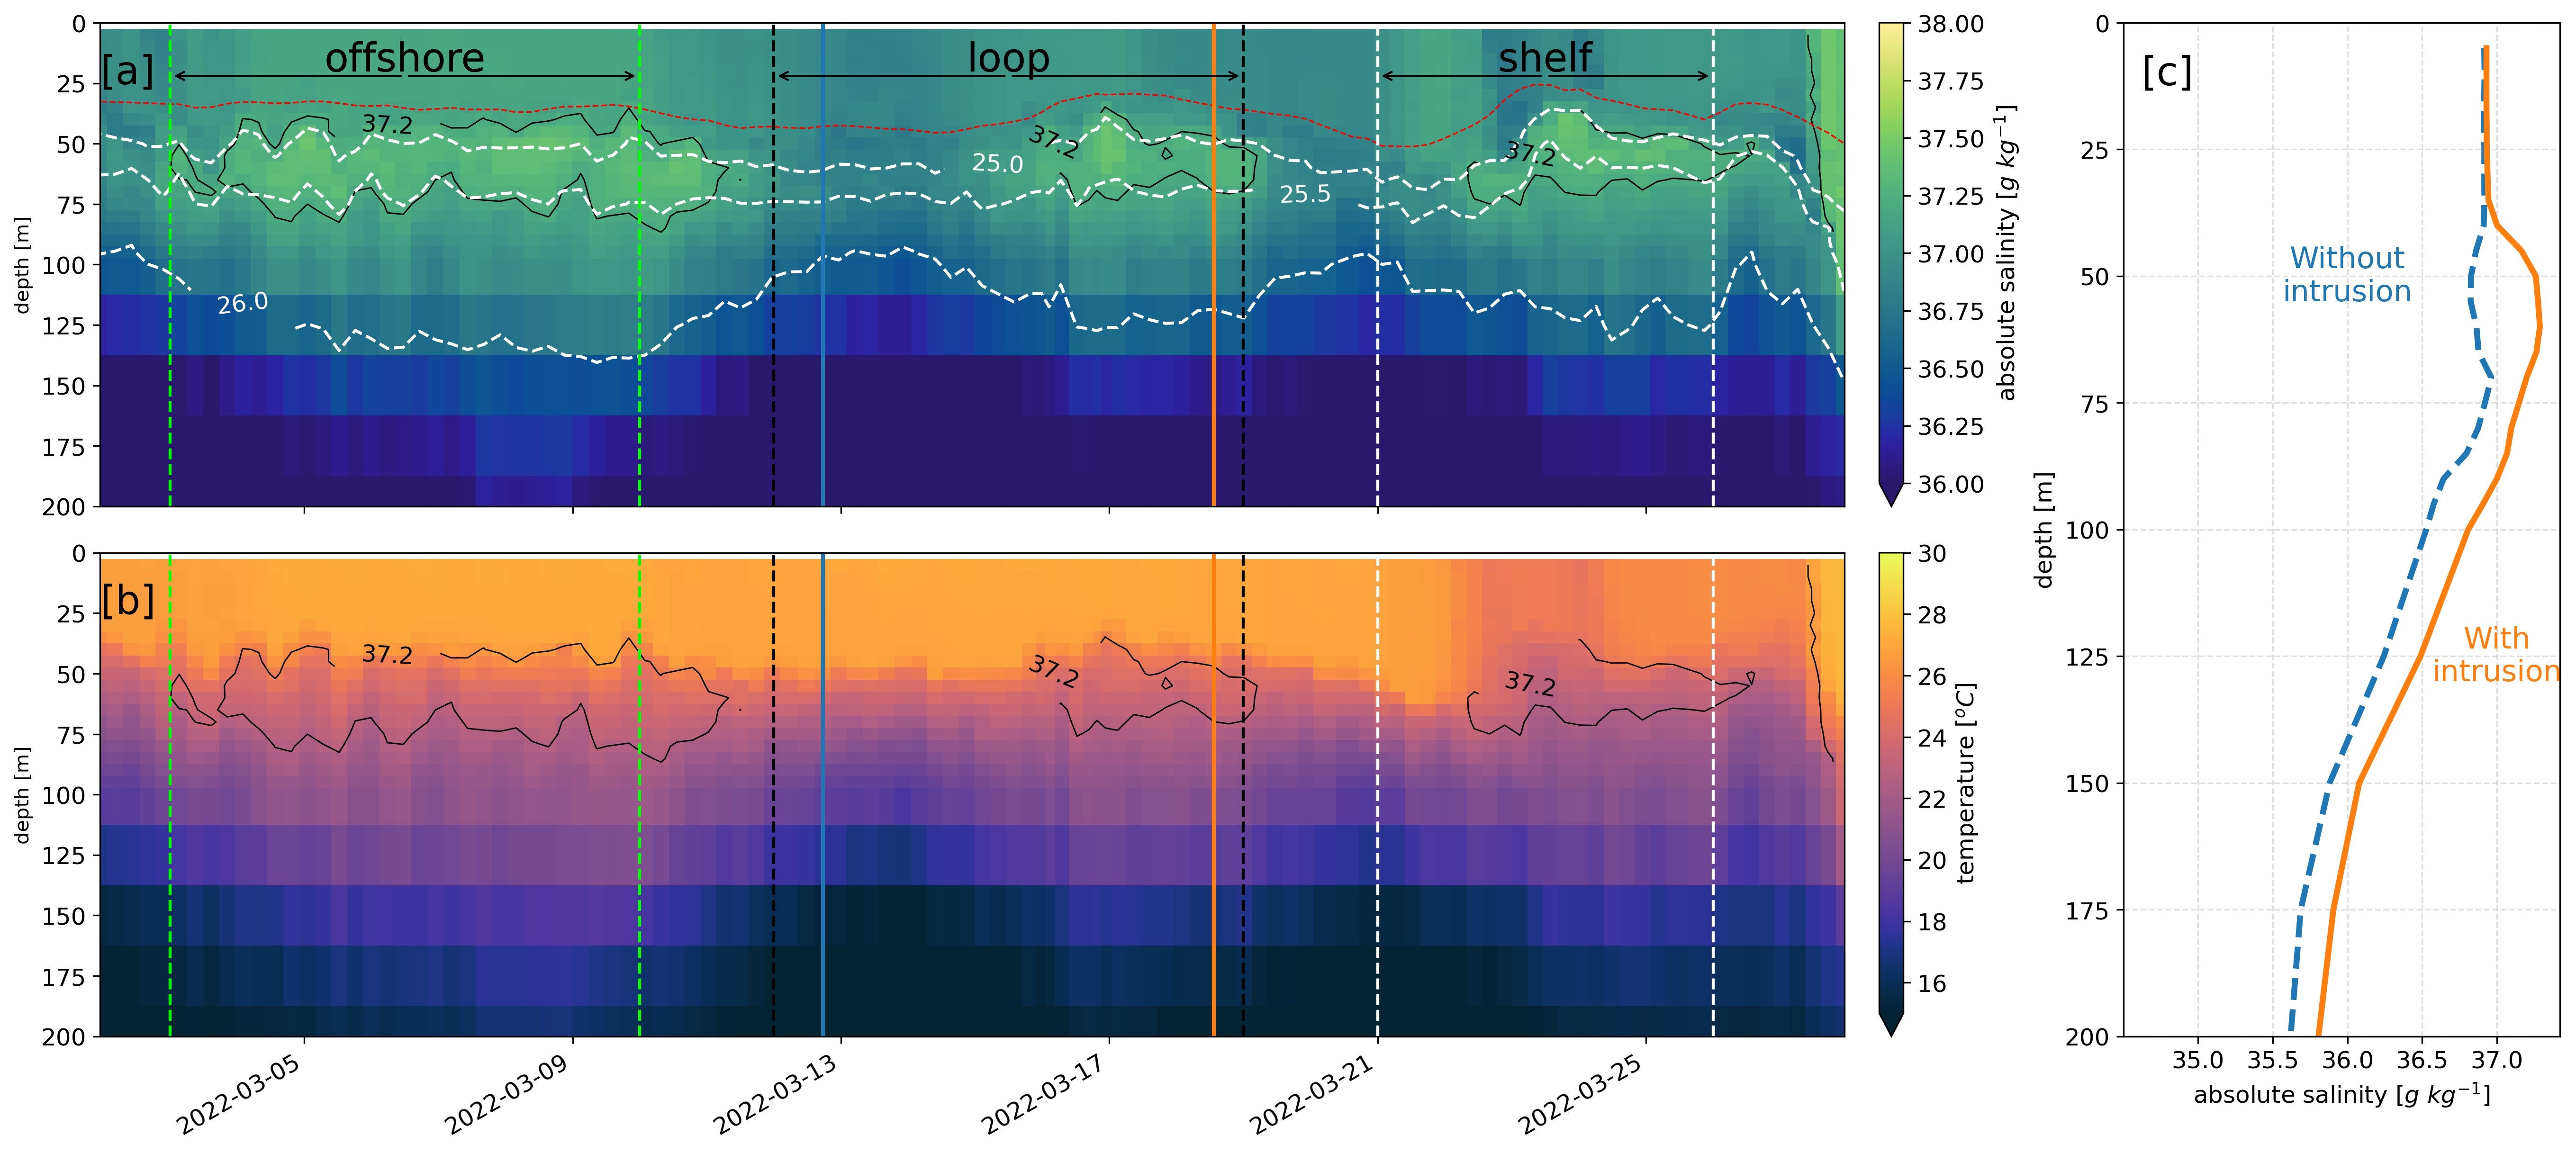
\includegraphics[width=1\linewidth]{figures/00_manuscript_glider_transect.png}
    \caption{Transects reconstructed from Slocum Glider SG19, for absolute salinity (top panel) and temperature (bottom panel) in (a). The black line indicates the 37.2 $g\ kg^{-1}$ isohaline, the white isopycnals for 25, 25.5 and 26 $kg\ m^{-3}$ and red dashed lines indicate the mixed layer depth, using the density criteria. The x-axis is time, while the y-axis is the depth in $m$. The path of the glider is shown in \protect Figure~\ref{fig:study_area} as a continuous black line. The green, black and white vertical dashed lines in (a) highlights periods where the \textit{$S_{max}$} was observed throughout the path, while the blue and orange continuous vertical lines represents the two profiles in (b), without and with the intrusions respectively.}
    \label{fig:glider_transect}
\end{figure}

In the first half (Figure~\ref{fig:glider_transect} a), the transect shows the presence of \textit{$S_{max}$} for this entire period, covering an extension of approximately 79 $km$. After this period, there was an absence of \textit{$S_{max}$} signal when the glider veered towards the shelf edge and to northeast, performing a loop pattern (Figure~\ref{fig:glider_transect} b), between 13$^{th}$ and 15$^{th}$ March. When the glider drifted westwards, between days 15 and 20, the salinity maximum was observed once again. Since the glider sampled almost the same location twice in a 6-day span (Figure~\ref{fig:study_area}, zoomed map), it is useful to explore the vertical profiles from these dives. For the first profile (Figure~\ref{fig:glider_transect} b, blue) we did not find any intrusion signal, using the \cite{silva2023inventory} methodology, but six days later the intrusion signal arrived at this location (Figure~\ref{fig:glider_transect} b, red). The effect of the \textit{$S_{max}$} increased the absolute salinity from 37 $g\ kg^{-1}$ to 37.4 $g\ kg^{-1}$, between 50 and 75 $m$ depth, but also had an influence in the water column, increasing the salinity from the mixed layer depth to, at least, 200 $m$ depth, by about 0.3 $g\ kg^{-1}$. Therefore, this second half of the glider dataset strengthens the suggestion of a \textit{$S_{max}$} advection towards the shelf edge. This becomes notably evident when examining the latter portion of the glider dataset (Figure~\ref{fig:glider_transect} c), spanning from the 22$^{nd}$ to the 25$^{th}$ March, during which the \textit{$S_{max}$} was once again detected, this time in closer proximity to the shelf edge.

\subsection{Water mass transformation}
\label{subsec:watermass}

We now select specific vertical profiles from the set of hydrographic data presented, that help describe the evolution of the \textit{$S_{max}$} via advection from deep waters to the NE-SBB (Figure~\ref{fig:train_profiles}). If we assume that the same \textit{$S_{max}$} was sampled across the datasets, it is possible to track the \textit{$S_{max}$} transformation with time and relate these changes to the main hydrodynamical processes in this region, like wind or eddy-driven circulation \cite{calado2010,uchoa2023,rocha2022,silveira2023}. See Figure~\ref{fig:train_profiles} f for the consecutive locations of profiles that have been traced chronologically to follow the advection of the salinity maximum intrusion from offshore to the shelf region of SBB.

In terms of water mass change throughout the profiles (Figure~\ref{fig:train_profiles} a to d), the \textit{$S_{max}$} presented salinity higher than 37 $g\ kg^{-1}$, associated to the presence of TW at the mixed layer, which is a salty and warm water mass \cite<S $\geq$ 37 $g\ kg^{-1}$ and $T$ $\geq$ 24$^o$C, >{cerda2014}, characteristic of the southwestern South Atlantic \cite{castro1998physical}. Note that the temperature in the first 3 profiles (Figure~\ref{fig:train_profiles} a to c) also shows warmer conditions, which have relevant impacts over the \textit{$S_{max}$} density. The salinity drops to 36.5 $g\ kg^{-1}$ and temperature decreases in about 4$^o$C once over the shelf (Figure~\ref{fig:train_profiles} d and e). The drop in salinity is probably related to the mixing with SACW, evidenced by the relatively colder waters \cite{cerda2014}. This is possible under upwelling favorable wind conditions, in which SACW is uplifted or upwelled, decreasing the temperature and salinity at the surface levels \cite{castro1998physical,cerda2014}. However, the amount of information is limited and does not allow us to infer the changes between the first and the second profiles. Nevertheless, these hydrographic conditions reveal the influence of local processes under the \textit{$S_{max}$} vertical position and the density associated with the maximum salinity.

\begin{figure}[ht!]
    \centering
    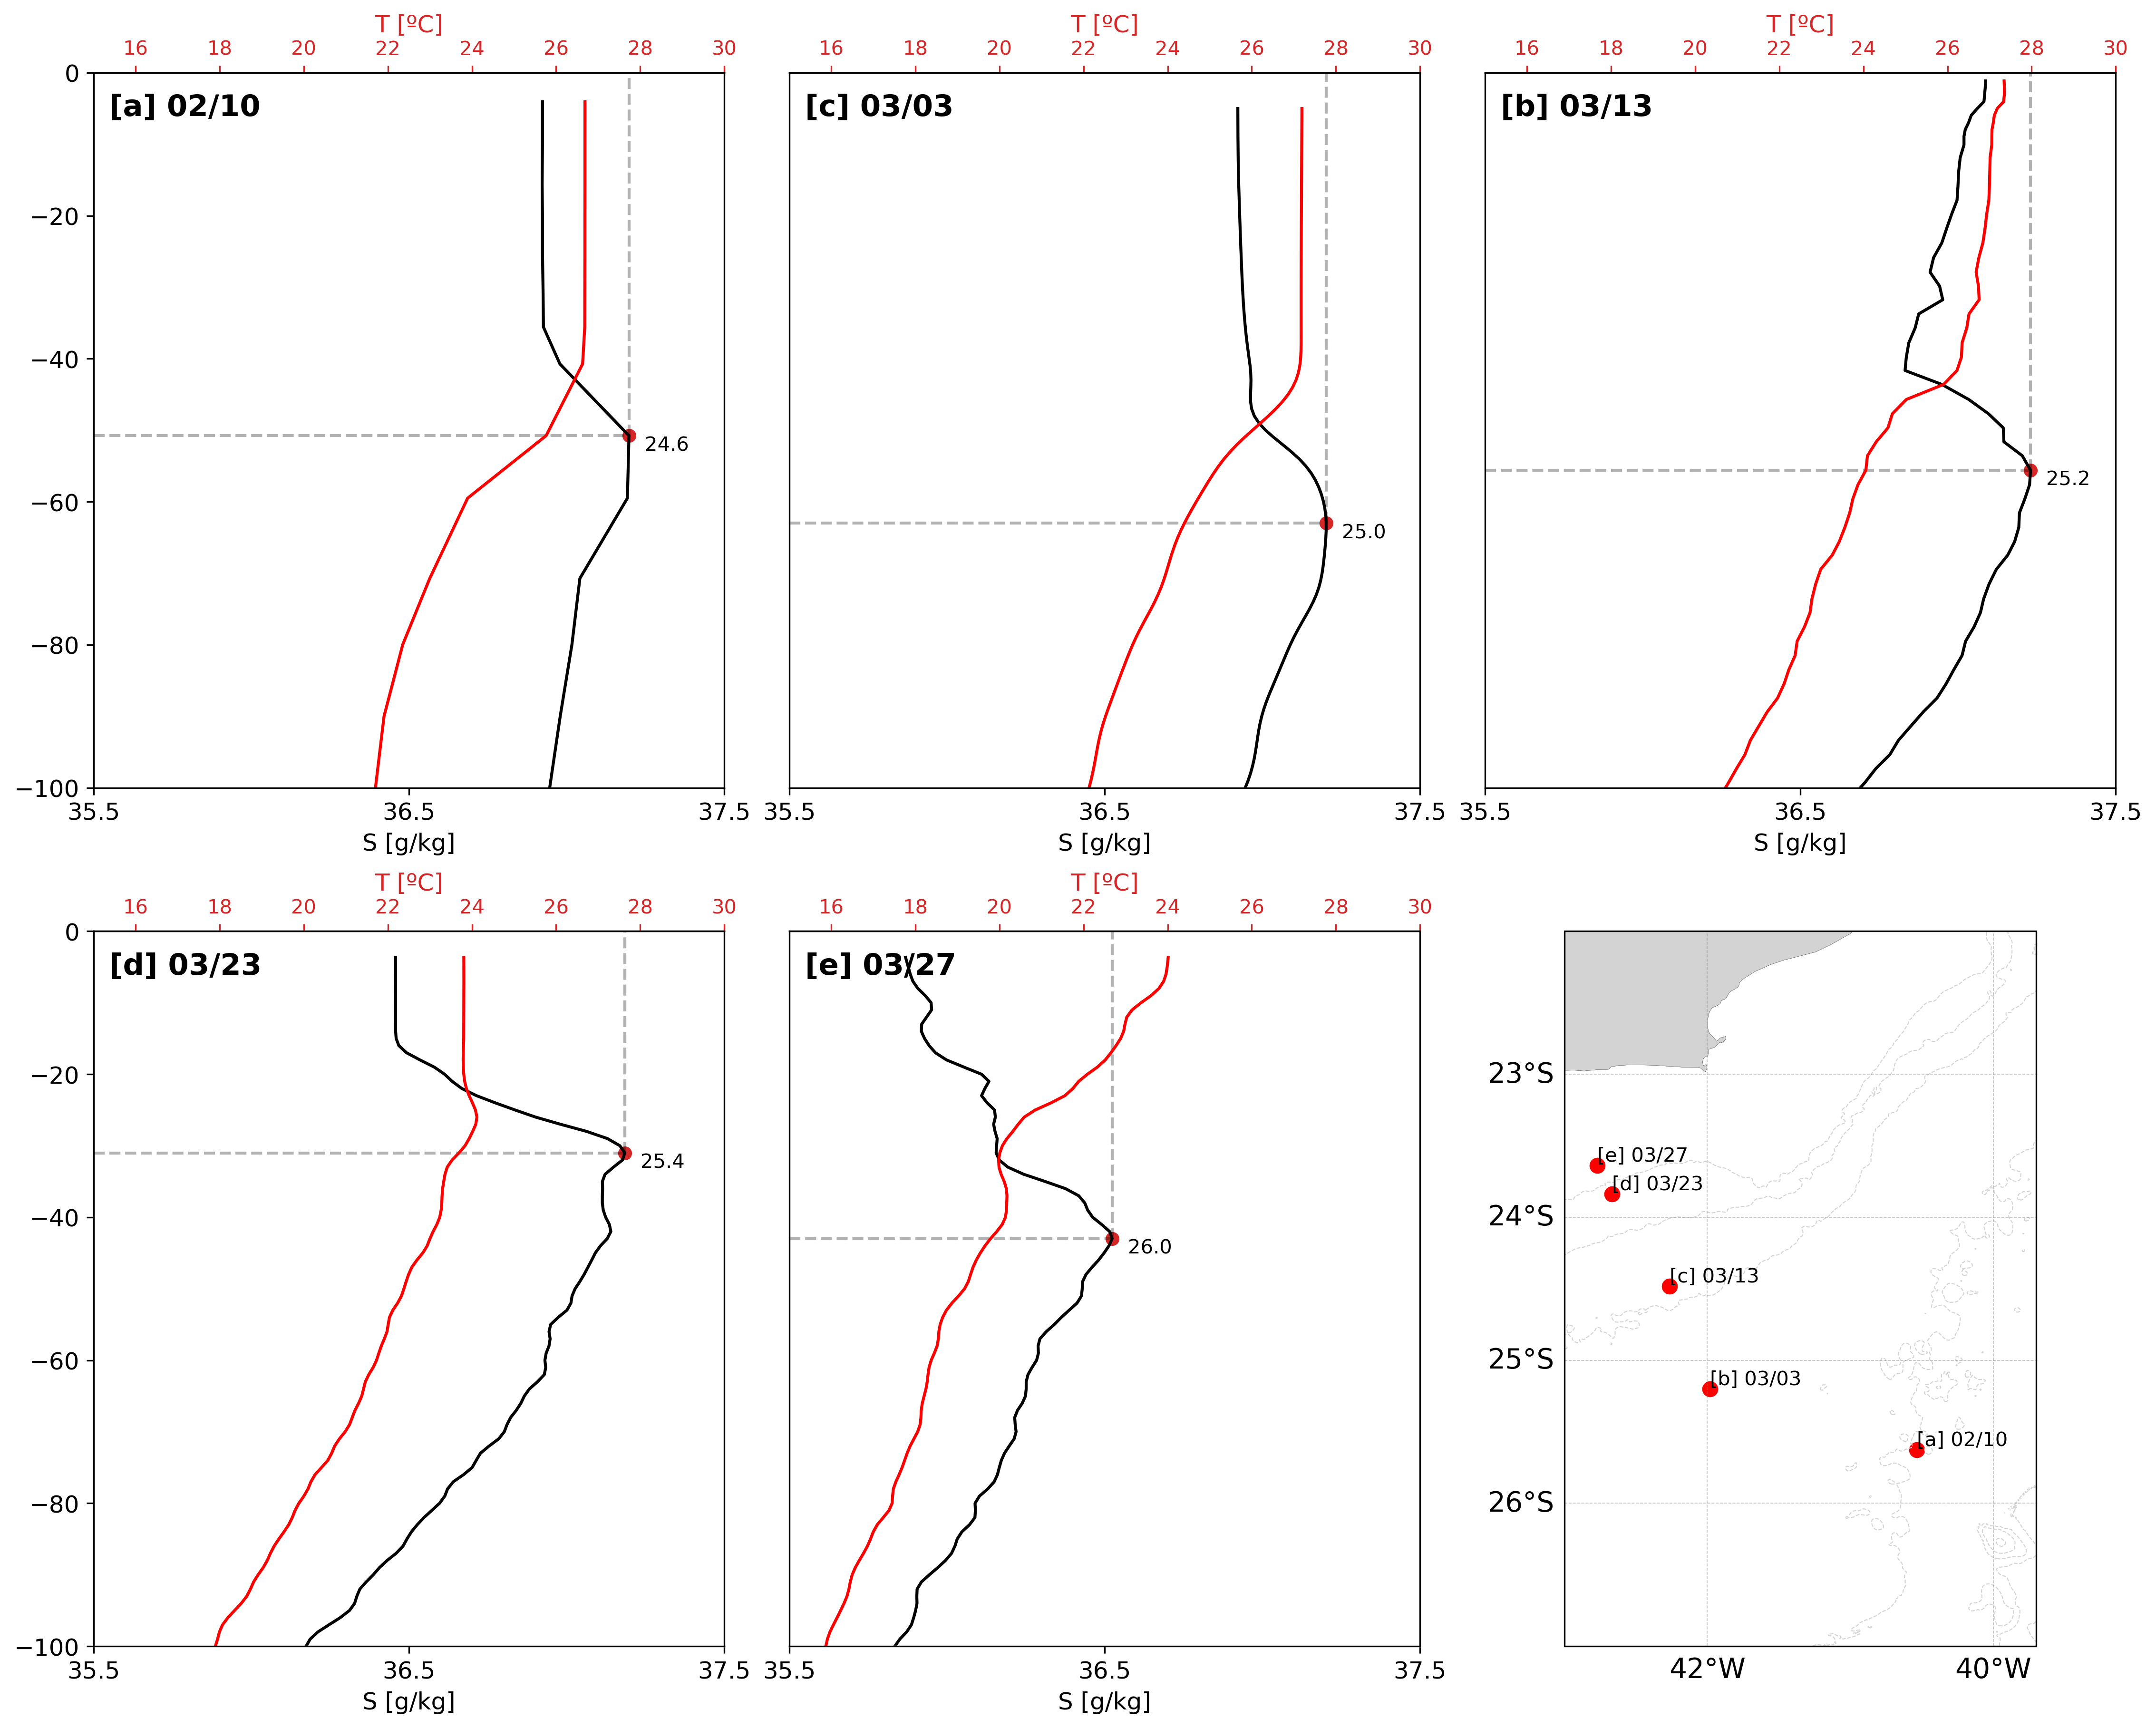
\includegraphics[width=0.8\linewidth]{figures/00_manuscript_train_profiles_new.png}
    \caption{Selected sequence of absolute salinity (black) and temperature (red) profiles with \textit{$S_{max}$} detected by the algorithm used by \protect\citeA{silva2023inventory}. Each vertical profile, from a to e, presents the depth of the \textit{$S_{max}$} as red marker along its potential density. In (f) there is the geographical position of each profile, along with their dates for reference.}
    \label{fig:train_profiles}
\end{figure}

\subsubsection{Lagrangian Pathways}
\label{subsec:lagpath}

The simulated particle transport pathways exhibit a set of significant cross-shelf components which can be advected either westwards, via a meandering pathway off NE-SBB, or by along-shelf advection over the 200-m isobath (Figure~\ref{fig:lagrangian_analysis} a) within a span of last 40 days. These results suggest two potential pathways for the advection of Smax: one originating from the east, with a higher probability, named as "cross-shelf pathway" hereafter, and the other, named "along-isobath pathway" originating from the north. 

The cross-shelf pathway holds the higher probability, accounting for 30$\%$ of the particles seeded over the shelf. It presents a meandering-like shape, swirling in the along shelf direction, but transporting particles effectively in the cross-shelf direction. There is a hotspot of particles centered at 42$^o$W and 25$^o$S, where the particles do not present a concise pathway, but an accumulation instead, even though a main path is still distinguishable. After 40 days, particles arrive in deeper regions, crossing isobaths, during advection reaching out from the 200 $m$ isobath to almost 4000 $m$ isobath. This Lagrangian analysis results presents a better fit with the selected vertical profiles used to understand the water mass transformation (Figure~\ref{fig:train_profiles}), as observed by the red dots in Figure~\ref{fig:lagrangian_analysis} a.

\begin{figure}[ht!]
    \centering
    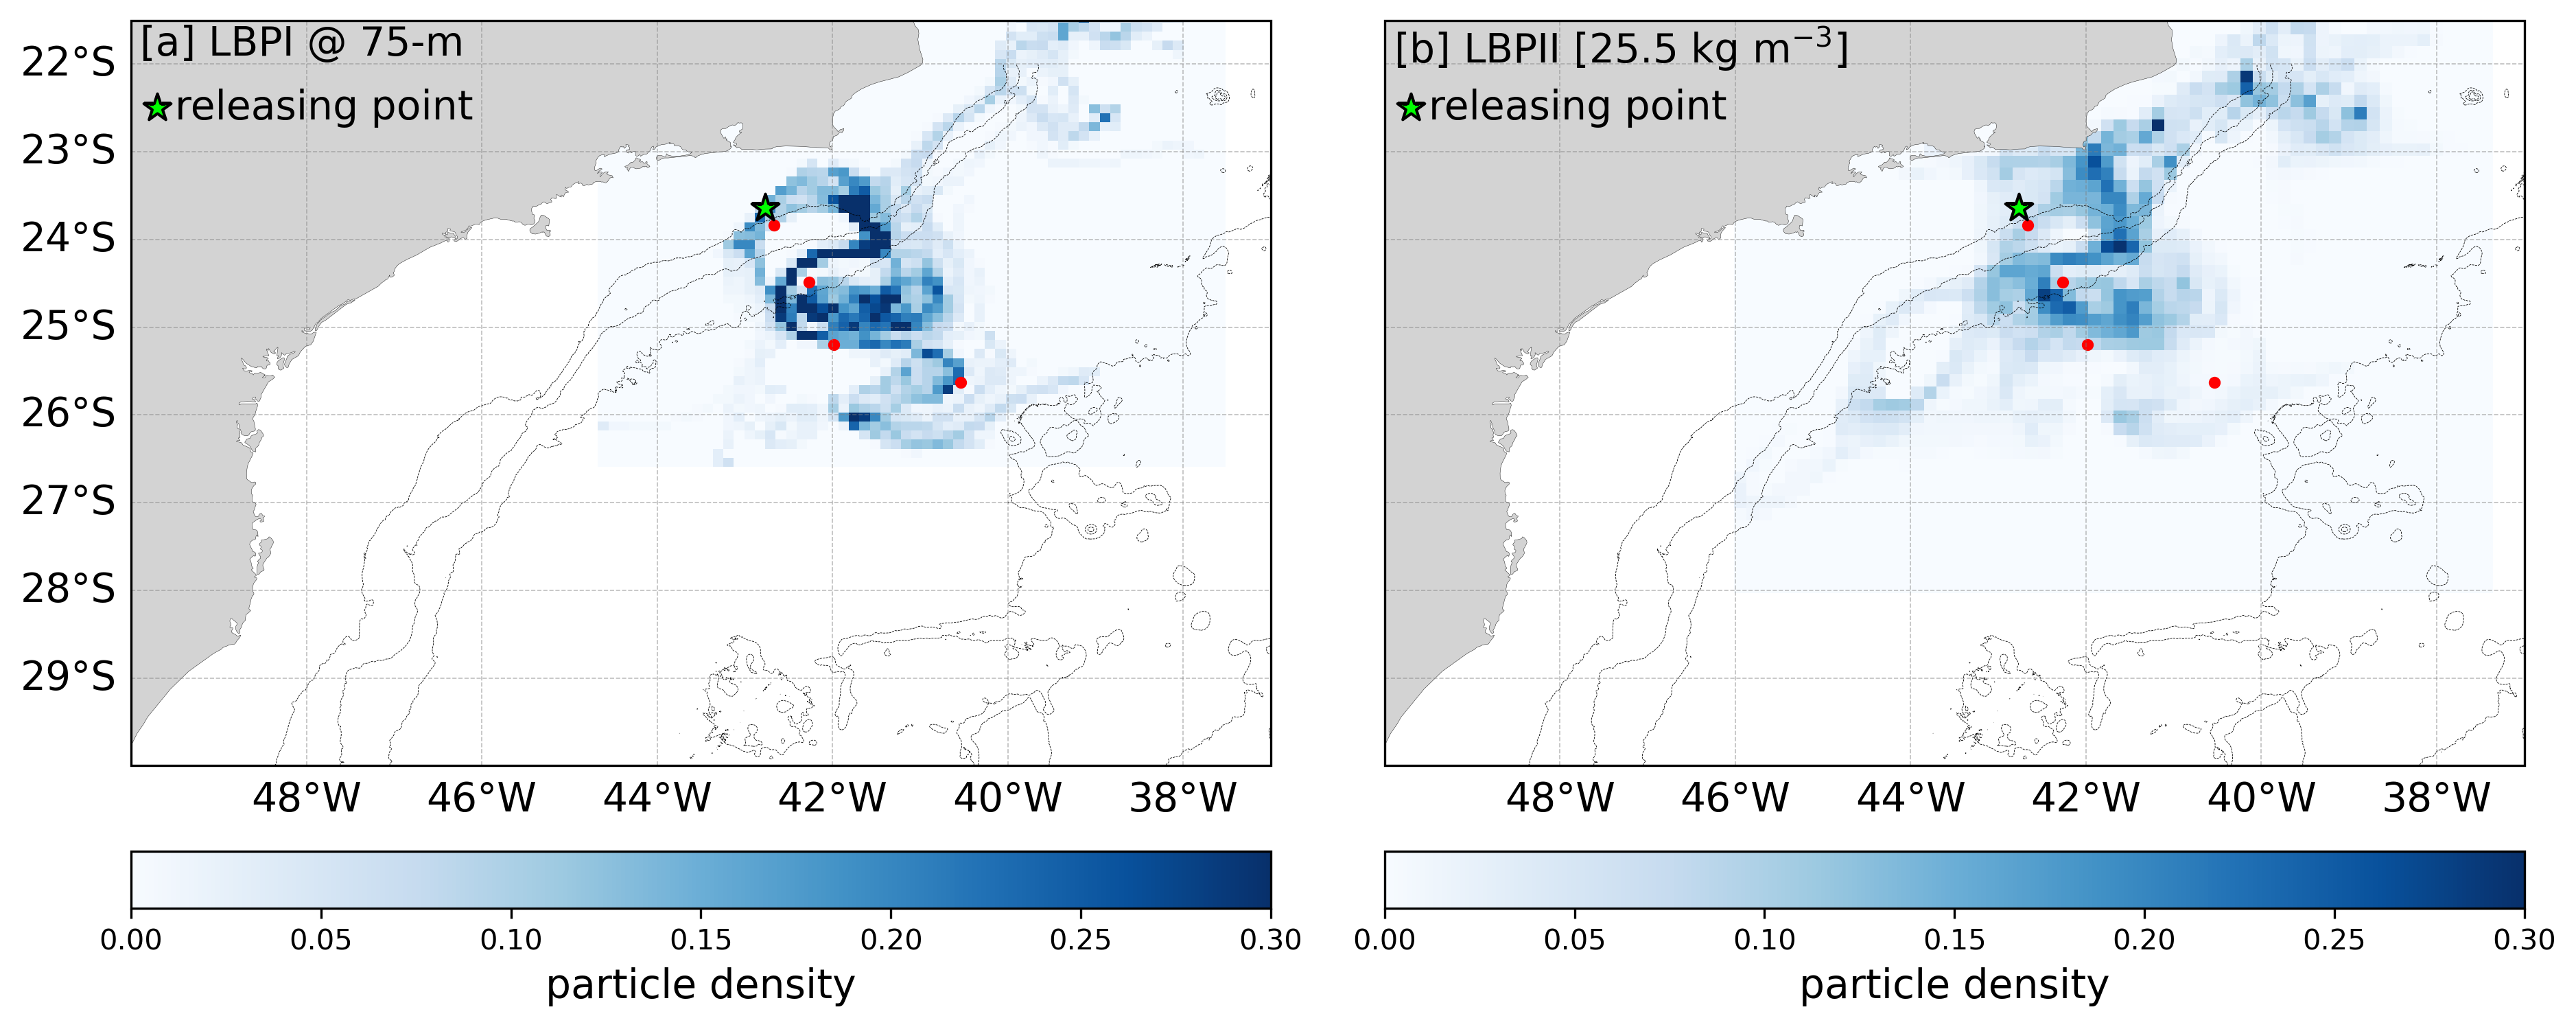
\includegraphics[width=1\linewidth]{figures/00_manuscript_lagrangian_analysis.png}
    \caption{Time integrated particles concentration on (a) the backpropagation experiment with releasing at the last \textit{$S_{max}$} observed in 27th March over the shelf at 50-m depth, (b) the forward propagation with releasing in 75-m depth at East and (c) at North. The red markers indicates the location of the sequence of profiles from \protect Figure~\ref{fig:train_profiles}.}
    \label{fig:lagrangian_analysis}
\end{figure}

Even though the east source seems to be the most probable origin of the March 2022 Smax, as shown by the cross-shelf pathway, a secondary source is identified from the back propagation analysis. The along-isobath pathway brings particles from the Tubarão Bight (28.25$^0$S), north of the region of interest (Figure~\ref{fig:lagrangian_analysis} a), transporting particles following the isobaths. However, over the region of interest, this pathway merges with the cross-shelf pathway and it is not possible to separate one from the other. To further understand the contribution/competition of each pathway, we performed two Lagrangian experiments, seeding particles at Southeast and Northeast of NE-SBB (Figure~\ref{fig:lagrangian_analysis} b and c, respectively), running forward in time.

Particle transports originating from the southeast, follow a cross-shelf pathway combined with eddy activity, towards the NE-SBB (Figure~\ref{fig:lagrangian_analysis} b). The pathway splits in two, one advecting particles towards open ocean (southeast) and another transporting particles in an anticyclonic pattern. This second pathway also concentrates the higher density of particles within the anticyclone, corresponding to almost 30$\%$ of the particles released. However, almost 10$\%$ of the particles detach towards the shelf, describing a cyclonic gyre near the 1000 $m$ isobath. After that, particles are transported towards the 200$m$ isobath in two separate pathways: one that tends to flow along the isobaths southwestwards and another that flows cross-isobath, towards the NE-SBB. This cross-isobath pathway is consistent with observations from the selected vertical profiles (Figure~\ref{fig:train_profiles}) and is consistent with the back propagation cross-shelf pathway (Figure~\ref{fig:lagrangian_analysis} a). We highlight the cyclonic behavior near the shelf edge corresponds to the same region where the Slocum Glider track turned cyclonically (Figure~\ref{fig:study_area}).

Particles from Northeast following the isobaths present a pathway near to the shelf break that follows the isobaths (Figure~\ref{fig:lagrangian_analysis} c). This pathway seems to be bounded between the 200 and 1000 $m$ isobaths and it is responsible for transporting particles throughout the entire SBB. Over the shelf orientation change in Cabo Frio, particles are slightly away from the 200 $m$ and then reattach again off Guanabara Bay (22.8$^0$S). This pattern is consistent with the meandering that leads to the development of the CFE and the cross-shelf transport generated from this meandering occurs at the same region in which \textit{$S_{max}$} signals were identified in vertical profiles. However, particles are advected further southwest, passing by the NB-SBB, reaching the SBB central area (43.5$^o$W; 25.5$^o$S), where higher accumulation of particles are consistent with anticyclonic patterns in this region \cite{silveira2023}.

\subsection{Ekman Transport on the Shelf}
\label{sub:ekman}

The surface ekman transport ($T_{Ek}$), computed from wind stress, is presented in Figure S2 as vectors. It shows that throughout the first observational cruise, $T_{Ek}$ was predominantly offshelf (Figure S2 a), due to constant northeasterly winds, from the South Atlantic Subtropical High \cite<SASH, >{stech1990estudo}, generating an offshelf Ekman Transport of approximately 80 $m^3\ s^{-1}$. Even though winds from SASH are mild \cite{stech1990estudo}, its persistence drives significant cross-shelf exchanges, pushing cold and nutrient-richs waters (SACW) towards the surface. It results in coastal upwelling such as the one observed during SANAGU14, also generating a cross-shelf SST gradient (Figure S1 a). Between SANAGU14 and SANAGU15, the wind pattern inverted and intensified, due to a cold front passage \cite{stech1990estudo}. It not only affected the sea surface by increasing the input of momentum, but also affected the incident solar radiation by developing a cloud coverage, which reduced the SST observed later on (Figure S1 b). However, the wind inversion was not persistent enough to generate an onshelf surface $T_{Ek}$ (not shown), resulting only in relatively weaker offshelf $T_{Ek}$, reducing from 50 $m^3\ s^{-1}$ between the cruises (Figure S2 b) to 20 $m^3\ s^{-1}$ in the second cruise (Figure S2 c).

% TODO: checar conteudo abaixo para finalizar
Onshelf transport, in response to the offshelf Ekman transport at the surface, occurs in depth, in which can be either near the bottom or in mid-waters \cite{LentzChapman2004}. During the period analyzed, the onshelf transport over the shelf edge was above the bottom Ekman layer, i.e., in subsurface levels, as pointed out by the Burger number ($Bu$) higher than 1 \cite{LentzChapman2004}, computed using the observed vertical profiles from SANAGU14 and SANAGU15 (Table~\ref{tab:burger_number}).

\begin{table}[ht!]
\label{tab:burger_number}
\caption{Summary of topographic gradient ($\alpha$), Buoyancy Frequency ($N^2$) and Burger number ($Bu$, \ref{eq:burger}) computed for specific CTD profiles extracted from SANAGU14 and SANAGU15 campaings.}
\centering
\begin{tabular}{c c c c}
\hline
\textbf{Vertical profile} & \textbf{$\alpha$} & \textbf{$N^2 [s^{-1}]$} & \textbf{$Bu$} \\
\hline
        SANAGU14 G4 & $23 \times 10^{-3}$ & $5.96 \times 10^{-5}$ & 9.15 \\
        SANAGU15 G4 & $23 \times 10^{-3}$ & $4.65 \times 10^{-5}$ & 7.14 \\
        SANAGU15 H4 & $11 \times 10^{-3}$ & $5.32 \times 10^{-5}$ & 2.16 \\
\hline
\multicolumn{2}{l}{$\alpha$ and $Bu$ are dimensionless numbers.}
\end{tabular}
\end{table}

\section{Discussion}
\label{section:discussion}

During the March 2022 campaign, multiple Salinity Maximum (\textit{$S_{max}$}) intrusions were observed off the Northeastern South Brazil Bight (NE-SBB). We found these signals are associated with the local stratification, occurring at the pycnocline, mainly between the 25 and 25.5 $kg\ m^{-3}$ isopycnals, and below the mixed layer (Figures~\ref{fig:cruise_transect},~\ref{fig:argo_alongshelf},~\ref{fig:argo_crossshelf},~\ref{fig:glider_transect}). The vertical extents of the salinity maximum intrusions are between the 50 and 75 $m$ depths, resulting in an average thickness of 25 $m$, consistent with the climatological 30-m thickness for \textit{$S_{max}$} intrusions in the NE-SBB \cite{silva2023inventory}. The salinity anomaly of 0.3 $g\ kg^{-1}$ spans between the summer (0.59 $g\ kg^{-1}$) and winter (0.34 $g\ kg^{-1}$) from the same climatology \cite{silva2023inventory}. 
However, due to the fact that \textit{$S_{max}$} in this period were located offshore, the maximum salinity values observed were higher than the ones described by \citeA{silva2023inventory} over the shelf: waters saltier than 37.1 $g\ kg^{-1}$ in observations over the deep ocean and 36 $g\ kg^{-1}$ over the shelf. These differences are expected, since freshwater from continental runoff influence in the NE-SBB does not reach regions further than the shelf break due to the low discharge in this area \cite{cerda2014,castro2014summer}. Thus, the SACW influence might act in the sense of reducing the salinity maximum near the surface, due to the coastal or eddy-driven upwelling \cite{Campos2000,cerda2014,castro2014summer}. \textit{$S_{max}$} intrusions, from the SBB, present similar properties to the ones from Middle Atlantic Bight \cite<MAB, >{Lentz2003}. In addition, particularly in the Northeast US shelf, \textit{$S_{max}$} intrusions are becoming more frequent since the 2000', associated with an increase in Warm Core Rings \cite{gangopadhyay2019observed,silver2023increased}, and penetrating larger distances shoreward \cite{gawarkiewicz2022increasing} relative to previous studies. The MAB \textit{$S_{max}$} intrusions are formed from the interaction between Warm Core Rings with the shelf break \cite{silver2023increased}, which could be a possible driving mechanism in the SBB as well.

Our investigation demonstrates the advection of \textit{$S_{max}$} intrusions from deeper ocean to the NE-SBB, predominantly via cross-shelf pathways, but also through along-shelf pathways, depending on the mesoscale dynamics (Figure~\ref{fig:lagrangian_analysis}). Figure~\ref{fig:schematic} summarizes the key pathways and components found in the AVISO geostrophic currents and Lagrangian analysis in a schematic. The observational dataset reveals the intrusion signals were found below the mixed layer in all observations (Section~\ref{sec:smax_structure}) which, in a first approximation, could be defined as the maximum depth where atmospheric processes play a role on the hydrodynamics \cite{giunta2022ocean}. Thus, it is reasonable to assume that the mesoscale dynamical processes were responsible for the advection of the \textit{$S_{max}$} signal towards the shelf edge.

During February and March 2022, the dataset presented here suggest the cross-shelf pathway as the main artery for the salty water-mass by that time (Figure~\ref{fig:lagrangian_analysis} a and b) and it can be sourced from two different pathways meeting at an offshore junction location near (41.5$^0$W, 25$^0$S). The first one is driven by northwestward geostrophic currents (see Figure~\ref{fig:geostrophic_fields} a for an example and Figure~\ref{fig:schematic} red solid line), advecting \textit{$S_{max}$} towards the shelf. During its advection, the \textit{$S_{max}$} achieves an unstable region, where the BC meanders, often necking off Cabo Frio Eddies \cite<CFE, >{rocha2022,uchoa2023,silveira2023}. In this confluence region for Smax, the \textit{$S_{max}$} appears to be captured by the BC meander (see Figure~\ref{fig:geostrophic_fields} a for an example and Figure~\ref{fig:schematic} dark blue solid line) and advected further towards the shelf edge. We cannot state clearly whether it is a BC meander or a cut off CFE, but the AVISO geostrophic fields analysis suggests the first case (Figure~\ref{fig:geostrophic_fields}). Thus, the second half of the cross-shelf pathway is driven by the BC meander. The along-shelf pathway contribution are not negligible and it represents a secondary source of \textit{$S_{max}$}, coming from North (Figure~\ref{fig:lagrangian_analysis} a and c). This pathway resembles the BC non meandering state (Figure~\ref{fig:schematic} dashed blue line), flowing along the isobaths, as it can be see in Figure~\ref{fig:geostrophic_fields} c. The BC, however, eventually become unstable and starts to meander, growing at an average rate of $0.1\ day^{-1}$ \cite<see Figure 3 in>{silveira2023}, until it reaches a state of necking off a CFE \cite{uchoa2023}. In this case, the \textit{$S_{max}$} advection will present a cross-shelf pattern, similar to the meander at 24.5$^o$S and 42$^o$W in Figure~\ref{fig:schematic}. 

\begin{figure}[ht!]
    \centering
    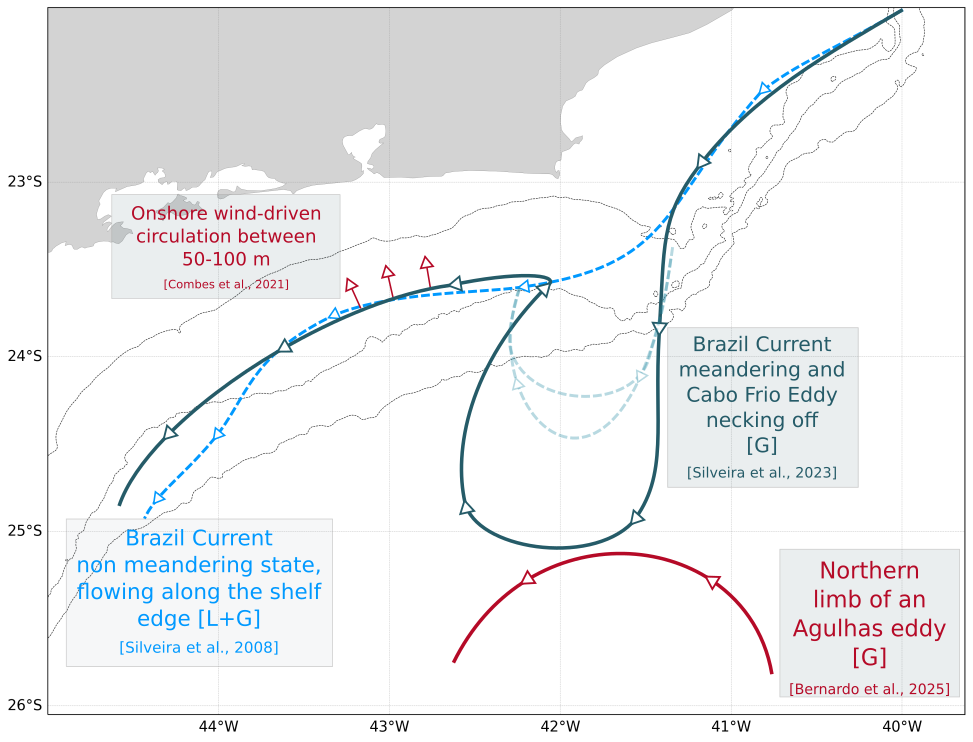
\includegraphics[width=1\linewidth]{figures/pathways_schematics_structure.png}
    \caption{Schematic flow field summarizing the three pathways scenarios of Salinity Maximum intrusions, obtained from the jointly analysis of the geostrophic fields (G, Figure~\ref{fig:geostrophic_fields}) and lagrangian outputs (L, Figure~\ref{fig:lagrangian_analysis}). The cross-shelf pathway is a combination of northwestward geostrophic currents (red) and the meandering state of the Brazil Current (dark blue), while the along-shelf edge pathway is given in dashed light blue.}
    \label{fig:schematic}
\end{figure}

Exchange between sea and open ocean are often ageostrophic, since geostrophic currents are constrained to flow along isobaths \cite{brink2016}. Thus, geostrophy might enhance cross-shelf edge dynamics, but ageostrophic processes will dominate them. For instance, it has been shown that mesoscale eddies enhance the shelf sea exchange \cite{mizobata2006,Malan2020,rautenbach2023,eshghi2023impact} and that might be the case of the SBB \textit{$S_{max}$}. At the NE-SBB, wind-driven cross-shelf exchanges are found from 50 $m$ to 100 $m$ \cite{combes2021circulation}, promoting onshelf advection in the presence of northeasterly winds (upwelling-favorable winds), which was the case during the period of interest (see Ekman transport in Figure S2). The Burger number ($Bu$, Table~\ref{tab:burger_number}) corroborates the pattern expected, suggesting a preferential cross-shelf pathway occurring in mid-depth during the campaigns, as indicated by values higher than 1 \cite{LentzChapman2004}. Even though this response might be affected by eddies \cite{castelao2006upwelling}, the data analysis performed here shows that the BC meander potentially enhance the shoreward wind-driven circulation during the period of interest (Figure S3). However, our dataset does not allow us to further understand the interplay of these processes, demanding numerical experiments carefully designed to this end \cite<see >{wang2011,paloczy2016,Chen2019}.

\section{Concluding Remarks}
\label{section:concluding}

In this study, we present the first observational evidence of remotely advected Salinity Maximum (\textit{$S_{max}$}) intrusions in the Northeastern South Brazil Bight (NE-SBB). Using a multi-platform observational dataset, we tracked the pathway of \textit{$S_{max}$} from eastern locations off the NE-SBB to the continental shelf in this region. Our findings indicate that oceanic \textit{$S_{max}$} is consistent with those observed over the shelf \cite{silva2023inventory}, characterized by waters saltier than 37 g/kg and occurring between 50 and 100 meters depth. Since these intrusions exist below the mixed layer, their advection is primarily driven by geostrophic motion within the ocea's interior, as supported by Lagrangian analysis. For the case study examined, the dataset reveals a cross-shelf pathway, with \textit{$S_{max}$} advected from southeastern locations along northwestward geostrophic currents,  captured by a Brazil Current cyclonic meander, and further advected towards the shelf edge.

Lagrangian analysis corroborates this pathway and suggests an additional, likely secondary, along-shelf pathway, resembling the Brazil Current’s non-meandering state. Once over the shelf edge, the Burger number analysis indicates an onshore flow in mid-water in response to upwelling-favorable winds during the period, enhanced by mesoscale dynamics over the shelf edge. Thus, we suggest that the injection of \textit{$S_{max}$} onto the shelf is an interplay of wind- and eddy-driven  processes, although further work is needed to fully understand these mechanisms.

Our results shed light on the origins of \textit{$S_{max}$}, a less understood phenomenon in the SBB. Considering intrusions of salty and warm waters is crucial for better understanding the Cabo Frio upwelling system. Moreover, with climate change scenarios, further studies are necessary on the NE-SBB to comprehend the impacts of \textit{$S_{max}$} on the thermodynamics and biogeochemistry of this shelf.

%%%%%%%%%%%%%%%%%%%%%%%%%%%%%%%%%%%%%%%%%%%%%%%
%
% DATA SECTION and ACKNOWLEDGMENTS
%
%%%%%%%%%%%%%%%%%%%%%%%%%%%%%%%%%%%%%%%%%%%%%%%

\section*{Open Research Section}
The CTD casts, from the SANAGU campaing \cite{moreira2023multidisciplinary}, belongs to Petrobras and are not accesible to the public or research community. The ARGO profiles were obtained on April 2023 from the \textit{Institu Français de Recherche pour l'Explotation de la Mer} (IFREMER), via the ARGOPY package \cite<\url{https://joss.theoj.org/papers/10.21105/joss.02425}, >{Maze2020}. The Slocum Glider SG19 dataset are not accesible to the public or research community, but it is possible to request access via the ProjetoAzul website (\url{http://www.projetoazul.eco.br/}). The altimetry dataset were obtained on April 2023, from the Copernicus Marine Environment Monitoring Service (CMEMS), via their website: the Level 4 gridded product was accessed via \url{https://doi.org/10.48670/moi-00149} and the level 3 along track product was accessed via \url{https://doi.org/10.48670/moi-00146}. The wind stress product were obtained on April 2023, from the European Center for Medium-range Weather Forecast (ECMWF), via their website (\url{https://doi.org/10.24381/cds.adbb2d47}). The precipitation dataset from MERGE were obtained on April 2023, from the National Institute on Spatial Research (or INPE in Brazilian portuguese) website (\url{https://ftp.cptec.inpe.br/modelos/tempo/MERGE/GPM/DAILY/}). The sea surface temperature were obtained from the National Centers for Environmental Information (NCEI), via their website (\url{https://www.ncei.noaa.gov/data/oceans/pathfinder/Version5.3/L3C/}). All scripts used to reproduce the figures and analysis in this manuscript are available at \url{https://github.com/nilodna/smax_pathways/tree/v1.0.0}

\acknowledgments
We thank Petróleo Brasileiro S.A. (PETROBRAS) for their permission to use and display the proprietary data from Santos Project – Santos Basin Environmental Characterization – for this paper. The authors would like to thank all the organizations for making the dataset used in this research available. Danilo A. Silva and Dalton K. Sasaki acknowledge financial support from PETROBRAS (Santos Project, 2018/00068-8), Marcelo Dottori acknowledges support from the Fundação de Amparo à Pesquisa do Estado de São Paulo (FAPESP 2010/05124-1) and Ilson Carlos Almeida da Silveira acknowledges support from CNPq (Project HIDROSAN I, 405593/2021-0) and FAPESP (Project HIDROSAN II, 2021/13124-6). We also thank the reviewers for their valuable suggestions and comments, which considerably improved the quality of this article.


%%%%%%%%%%%%%%%%%%%%%%%%%%%%%%%%%%%%%%%%%%%%%%%
% REFERENCES and BIBLIOGRAPHY
\bibliography{references}
% \bibliography{<name of your .bib file>} don't specify the file extension
% don't specify bibliographystyle
%
%%%%%%%%%%%%%%%%%%%%%%%%%%%%%%%%%%%%%%%%%%%%%%%
\end{document}



More Information and Advice:

%%%%%%%%%%%%%%%%%%%%%%%%%%%%%%%%%%%%%%%%%%%%%%%
%
%  SECTION HEADS
%
%%%%%%%%%%%%%%%%%%%%%%%%%%%%%%%%%%%%%%%%%%%%%%%

% Capitalize the first letter of each word (except for
% prepositions, conjunctions, and articles that are
% three or fewer letters).

% AGU follows standard outline style; therefore, there cannot be a section 1 without
% a section 2, or a section 2.3.1 without a section 2.3.2.
% Please make sure your section numbers are balanced.
% ---------------
% Level 1 head
%
% Use the \section{} command to identify level 1 heads;
% type the appropriate head wording between the curly
% brackets, as shown below.
%
%An example:
%\section{Level 1 Head: Introduction}
%
% ---------------
% Level 2 head
%
% Use the \subsection{} command to identify level 2 heads.
%An example:
%\subsection{Level 2 Head}
%
% ---------------
% Level 3 head
%
% Use the \subsubsection{} command to identify level 3 heads
%An example:
%\subsubsection{Level 3 Head}
%
%---------------
% Level 4 head
%
% Use the \subsubsubsection{} command to identify level 3 heads
% An example:
%\subsubsubsection{Level 4 Head} An example.
%
%%%%%%%%%%%%%%%%%%%%%%%%%%%%%%%%%%%%%%%%%%%%%%%
%
%  IN-TEXT LISTS
%
%%%%%%%%%%%%%%%%%%%%%%%%%%%%%%%%%%%%%%%%%%%%%%%
%
% Do not use bulleted lists; enumerated lists are okay.
% \begin{enumerate}
% \item
% \item
% \item
% \end{enumerate}
%
%%%%%%%%%%%%%%%%%%%%%%%%%%%%%%%%%%%%%%%%%%%%%%%
%
%  EQUATIONS
%
%%%%%%%%%%%%%%%%%%%%%%%%%%%%%%%%%%%%%%%%%%%%%%%

% Single-line equations are centered.
% Equation arrays will appear left-aligned.

Math coded inside display math mode \[ ...\]
 will not be numbered, e.g.,:
 \[ x^2=y^2 + z^2\]

 Math coded inside \begin{equation} and \end{equation} will
 be automatically numbered, e.g.,:
 \begin{equation}
 x^2=y^2 + z^2
 \end{equation}


% To create multiline equations, use the
% \begin{eqnarray} and \end{eqnarray} environment
% as demonstrated below.
\begin{eqnarray}
  x_{1} & = & (x - x_{0}) \cos \Theta \nonumber \\
        && + (y - y_{0}) \sin \Theta  \nonumber \\
  y_{1} & = & -(x - x_{0}) \sin \Theta \nonumber \\
        && + (y - y_{0}) \cos \Theta.
\end{eqnarray}

%If you don't want an equation number, use the star form:
%\begin{eqnarray*}...\end{eqnarray*}

% Break each line at a sign of operation
% (+, -, etc.) if possible, with the sign of operation
% on the new line.

% Indent second and subsequent lines to align with
% the first character following the equal sign on the
% first line.

% Use an \hspace{} command to insert horizontal space
% into your equation if necessary. Place an appropriate
% unit of measure between the curly braces, e.g.
% \hspace{1in}; you may have to experiment to achieve
% the correct amount of space.


%%%%%%%%%%%%%%%%%%%%%%%%%%%%%%%%%%%%%%%%%%%%%%%
%
%  EQUATION NUMBERING: COUNTER
%
%%%%%%%%%%%%%%%%%%%%%%%%%%%%%%%%%%%%%%%%%%%%%%%

% You may change equation numbering by resetting
% the equation counter or by explicitly numbering
% an equation.

% To explicitly number an equation, type \eqnum{}
% (with the desired number between the brackets)
% after the \begin{equation} or \begin{eqnarray}
% command.  The \eqnum{} command will affect only
% the equation it appears with; LaTeX will number
% any equations appearing later in the manuscript
% according to the equation counter.
%

% If you have a multiline equation that needs only
% one equation number, use a \nonumber command in
% front of the double backslashes (\\) as shown in
% the multiline equation above.

% If you are using line numbers, remember to surround
% equations with \begin{linenomath*}...\end{linenomath*}

%  To add line numbers to lines in equations:
%  \begin{linenomath*}
%  \begin{equation}
%  \end{equation}
%  \end{linenomath*}